
% Note for any github stalkers. I am currently in the process
% of learning LaTeX. I don't know what I'm doing yet. Sorry
% if my code absolutely sucks.


\documentclass{book}

\usepackage{fontspec} % used to import Calibri
\usepackage{anyfontsize} % used to adjust font size

% needed for inch and other length measurements
% to be recognized
\usepackage{calc}

% for colors and text effects as is hopefully obvious
\usepackage[dvipsnames]{xcolor}
\usepackage{soul}

% control over margins
\usepackage[margin=1in]{geometry}
\usepackage[strict]{changepage}

\usepackage{mathtools}
\usepackage{amsfonts}
\usepackage{amssymb} % originally imported to get the proof square
\usepackage{xfrac}

% Just am using this to get a dashed line in a table...
% Also you apparently want this to be inactive if you aren't
% using it because it slows compilation.
\usepackage{arydshln} \ADLinactivate 
\newenvironment{allowTableDashes}{\ADLactivate}{\ADLinactivate}

\usepackage{graphicx}
\graphicspath{{./158_Images/}}

\usepackage{tikz}
   \usetikzlibrary{arrows.meta}
   \usetikzlibrary{graphs, graphs.standard}

\newfontfamily{\calibri}{Calibri}
\setlength{\parindent}{0pt}
\definecolor{RawerSienna}{HTML}{945D27}


% Deprecated Text Commands (Don't use!!!)
% ~~~~~~~~~~~~~~~~~~~~~~~~~~~~~~~~~~~~~~~~~~~~~~~~~~~~
\newcommand{\hOneOld}{%
   \color{Black}%
   \fontsize{14}{14}\selectfont%
}
\newcommand{\hTwoOldd}{%
   \color{MidnightBlue}%
   \fontsize{13}{13}\selectfont%
}
\newcommand{\hThreeOld}{%
   \color{PineGreen}
   \fontsize{13}{13}\selectfont%
}
\newcommand{\hFourOldd}{%
   \color{Cerulean}
   \fontsize{12}{12}\selectfont%
}
\newcommand{\teachCommentOldd}{
   \color{Orange}%
   \fontsize{12}{12}\selectfont%
}
\newcommand{\exOneOldd}{%
   \color{Purple}%
   \fontsize{14}{14}\selectfont%
}
\newcommand{\exTwoOldd}{%
   \color{RedViolet}%
   \fontsize{13}{13}\selectfont%
}
\newcommand{\exPOldd}{%
   \color{VioletRed}%
   \fontsize{12}{12}\selectfont%
}
% Non Deprecated formatting commands use!!!
% ~~~~~~~~~~~~~~~~~~~~~~~~~~~~~~~~~~~~~~~~~~~~~~~~
\newcommand{\hOne}{%
   \color{Black}%
   \fontsize{14}{16}\selectfont%
}
\newcommand{\hTwo}{%
   \color{MidnightBlue}%
   \fontsize{13}{15}\selectfont%
}
\newcommand{\hThree}{%
   \color{PineGreen}
   \fontsize{13}{15}\selectfont%
}
\newcommand{\hFour}{%
   \color{Cerulean}
   \fontsize{12}{14}\selectfont%
}
\newcommand{\myComment}{%
   \color{RawerSienna}%
   \fontsize{12}{14}\selectfont%
}
\newcommand{\teachComment}{
   \color{Orange}%
   \fontsize{12}{14}\selectfont%
}
\newcommand{\exOne}{%
   \color{Purple}%
   \fontsize{14}{16}\selectfont%
}
\newcommand{\exTwo}{%
   \color{RedViolet}%
   \fontsize{13}{15}\selectfont%
}
\newcommand{\exP}{%
   \color{VioletRed}%
   \fontsize{12}{14}\selectfont%
}
% ~~~~~~~~~~~~~~~~~~~~~~~~~~~~~~~~~~~~~~~~~~~~~~~~

\newcommand{\cyPen}[1]{{\vphantom{.}\color{Cerulean}#1}}

\newenvironment{myIndent}{%
   \begin{adjustwidth}{2.5em}{0em}%
}{%
   \end{adjustwidth}%
}

\newenvironment{myDindent}{%
   \begin{adjustwidth}{5em}{0em}%
}{%
   \end{adjustwidth}%
}

\newenvironment{myTindent}{%
   \begin{adjustwidth}{7.5em}{0em}%
}{%
   \end{adjustwidth}%
}

\newenvironment{myConstrict}{%
   \begin{adjustwidth}{2.5em}{2.5em}%
}{%
   \end{adjustwidth}%
}

\newcommand{\udefine}[1]{{%
   \setulcolor{Red}%
   \setul{0.14em}{0.07em}%
   \ul{#1}%
}}

\newcommand{\uuline}[2][.]{%
{\vphantom{a}\color{#1}%
\rlap{\rule[-0.18em]{\widthof{#2}}{0.06em}}%
\rlap{\rule[-0.32em]{\widthof{#2}}{0.06em}}}%
#2}

\newcounter{LectureNumber}
\newcommand*{\markLecture}[1]{%
   \stepcounter{LectureNumber}%
   {\huge \color{Black} \textbf{Lecture \theLectureNumber: #1} \newline}%
}

\newcommand{\pprime}{\prime\prime}
\newcommand{\suchthat}{ \hspace{0.5em}s.t.\hspace{0.5em}}
\newcommand{\rea}[1]{\mathrm{Re}(#1)}
\newcommand{\ima}[1]{\mathrm{Im}(#1)}
\newcommand{\comp}{\mathsf{C}}
\newcommand{\oddComp}[1]{\mathrm{odd}(#1)}
\newcommand{\exposed}[1]{\mathrm{ex}(#1)}
\newcommand{\exNums}[1]{\mathrm{ex}(#1)}
\newcommand{\myHS}{ \hspace{0.5em}}

% Thank you Gonzalo Medina and Moriambar who wrote this on stack exchange:
%https://tex.stackexchange.com/questions/74125/how-do-i-put-text-over-symbols%
\newcommand{\myequiv}[1]{\stackrel{\mathclap{\normalfont\mbox{\footnotesize#1}}}{\equiv}}

% Thank you chs who wrote this on stack exchange:
%https://tex.stackexchange.com/questions/89821/how-to-draw-a-solid-colored-circle%
\newcommand{\filledcirc}[1][.]{\ensuremath{\hspace{0.05em}{\color{#1}\bullet}\mathllap{\circ}\hspace{0.05em}}}

\newcounter{PropNumber}
\newcommand{\propCount}{%
   \stepcounter{PropNumber}%
   \thePropNumber%
}

\newcommand{\mySepOne}[1][.]{%
   {\noindent\color{#1}{\rule{6.5in}{1mm}}}\\%
}
\newcommand{\mySepTwo}[1][.]{%
   {\noindent\color{#1}{\rule{6.5in}{0.5mm}}}\\%
}

\newenvironment{myClosureDeprecated}[2][.]{%
   \color{#1}%
   \begin{tabular}{|p{#2in}|} \hline \\%
}{%
   \\ \\ \hline \end{tabular}%
}

\newenvironment{myClosureOne}[2][.]{%
   \color{#1}%
   \begin{tabular}{|p{#2in}|} \hline \\%
}{%
   \\ \hline \end{tabular}%
}

\newcommand{\retTwo}{\hfill\bigbreak}

\newcommand{\gfam}[1]{\mathcal{#1}}

\title{Math 158 Lecture Notes (Professor: Jacques Verstraete)}
\author{Isabelle Mills}


\begin{document}
   \maketitle
   \calibri

   \markLecture{1/9/2024}

   \hOneOld
   A \udefine{graph} is a pair $(V, E)$ where $V$ is a set of vertices
   and $E$ is a set of unordered pairs of elements of $V$ called edges.
   For $u, v \in V$, we say $u$ and $v$ are \udefine{adjacent} if 
   $\{u, v\} \in E$.

   
   \begin{center}
      \hTwoOldd
      For example: $G = (\{1, 2, 3\}, \{\{1, 2\}, \{2, 3\}\})$
      
      % I'm so sorry I'm not using the packages I should be using
      % to draw these graphs. I haven't had time to learn them yet
      % and I want this section done at some point tonight before I go
      % to bed. 
      \hThreeOld
      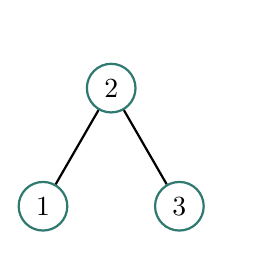
\begin{tikzpicture}
         \useasboundingbox (225:1.5) rectangle (45:2.5);

         \node (2) at (90:1) [circle, 
            draw=PineGreen!70!MidnightBlue, thick, fill=White] {2};
         \node (1) at (210:1) [circle, 
            draw=PineGreen!70!MidnightBlue, thick, fill=White] {1};
         \node (3) at (330:1) [circle, 
            draw=PineGreen!70!MidnightBlue, thick, fill=White] {3};
         \draw [thick] (1) -- (2);
         \draw [thick] (2) -- (3);
      \end{tikzpicture}
   \end{center}

\hOneOld
A \udefine{directed graph} (a.k.a a \udefine{digraph}) is a pair $(V, E)$ 
where $V$ is a set of vertices and $E$ is a set of ordered pairs 
of elements of $V$.
\begin{center}
   \hTwoOldd
   For example: $G = (\{1, 2, 3\}, \{(1, 2), (2, 3)\})$

   \hThreeOld
   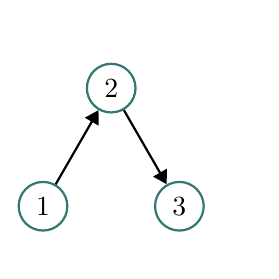
\begin{tikzpicture}
      \useasboundingbox (225:1.5) rectangle (45:2.5);

      \node (2) at (90:1) [circle, 
         draw=PineGreen!70!MidnightBlue, thick, fill=White] {2};
      \node (1) at (210:1) [circle, 
         draw=PineGreen!70!MidnightBlue, thick, fill=White] {1};
      \node (3) at (330:1) [circle, 
         draw=PineGreen!70!MidnightBlue, thick, fill=White] {3};
      \draw [thick, -Triangle] (1) -- (2);
      \draw [thick, -Triangle] (2) -- (3);
   \end{tikzpicture}
\end{center}

\hOneOld
A \udefine{multigraph} is a pair $(V, E)$ where $V$ is a set of vertices
and $E$ is a multiset of unordered pairs of elements of $V$.

\begin{center}
   \hTwoOldd
   For example: $G = (\{1, 2, 3\}, \{\{1, 2\}, \{2, 3\}, \{2, 3\}\})$
   
   \hThreeOld
   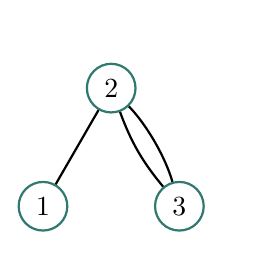
\begin{tikzpicture}
      \useasboundingbox (225:1.5) rectangle (45:2.5);

      \node (2) at (90:1) [circle, 
         draw=PineGreen!70!MidnightBlue, thick, fill=White] {2};
      \node (1) at (210:1) [circle, 
         draw=PineGreen!70!MidnightBlue, thick, fill=White] {1};
      \node (3) at (330:1) [circle, 
         draw=PineGreen!70!MidnightBlue, thick, fill=White] {3};
      \draw [thick] (1) -- (2);
      \draw [thick] (2) .. controls (50:.7) and (10:.7) .. (3);
      \draw [thick] (2) .. controls (50:.4) and (10:.4) .. (3);
   \end{tikzpicture}
\end{center}

\hOneOld
A \udefine{pseudograph} is like a graph and multigraph except that the
pairs in $E$ are multisets. 
\begin{myIndent}\begin{myIndent}\begin{myIndent}
\begin{myIndent}\begin{myIndent}
   \teachCommentOldd
   Essentially, an element $\{a, a\}$ can belong to $E$ in a 
   \\pseudograph. This type of edge is called a \udefine{loop}.
\end{myIndent}\end{myIndent}\end{myIndent}
\end{myIndent}\end{myIndent}

\begin{center}
   \hTwoOldd
   For example: $G = (\{1, 2, 3\}, \{\{1, 2\}, \{2, 3\}, \{3, 3\}\})$
   
   \hThreeOld
   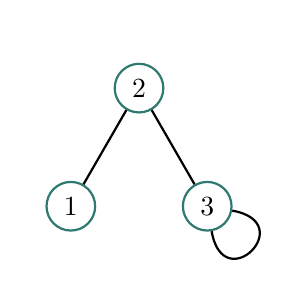
\begin{tikzpicture}
      \useasboundingbox (225:2) rectangle (45:2.5);

      \node (2) at (90:1) [circle, 
         draw=PineGreen!70!MidnightBlue, thick, fill=White] {2};
      \node (1) at (210:1) [circle, 
         draw=PineGreen!70!MidnightBlue, thick, fill=White] {1};
      \node (3) at (330:1) [circle, 
         draw=PineGreen!70!MidnightBlue, thick, fill=White] {3};
      \draw [thick] (1) -- (2);
      \draw [thick] (2) -- (3);
      \draw [thick] (3) to [out=350,in=280,looseness=6] (3);
   \end{tikzpicture}
\end{center}

\newpage
\hOneOld
If $G = (V, E)$ and $v \in V$, the \udefine{neighborhood} of $v$ is
$N_{G}(v)=\{w \in V \mid \{v, w\} \in E\}$. \bigbreak

The \udefine{degree} of $v$ is $d_{G}(v) = \lvert N_{G}(v) \rvert$.
Or in other words, $v$'s degree is equal to the number of edges 
connecting to $v$.

\mySepTwo[MidnightBlue]
\hTwoOldd
\begin{myIndent}
   The \udefine{Handshaking lemma} states that for any graph $(V, E)$:
      {\fontsize{16}{15}\selectfont
      \[ \sum_{v \in V} d_{G}(v) = 2 \lvert E \rvert \]}
   
   \hThreeOld
   \begin{myIndent}
      The reason for this is that each edge increments the degrees of
      exactly two vertices. So the above sum counts every edge twice.
      \hfill \bigbreak
   \end{myIndent}

   \hTwoOldd
   \uuline{Lemma}: Every graph has an even number of vertices with odd
   degrees.

   \hThreeOld
   \begin{myIndent}
      Proof: We can split the vertices of any graph into two categories:
      those with odd degrees, and those with even degrees.
      \hfill \bigbreak
      Now recall that an even number plus an even number always equals
      an even number, as does an odd number plus an odd number. However,
      an odd\\ number plus an even numbers equals an odd number. Based on
      this fact, we can guarentee that the sum of even degrees in any
      graph is even. And since the sum of even degrees plus the sum of 
      odd degrees must be even as it equals $2 \lvert E \rvert$ by
      the Handshaking lemma, we thus know that the sum of odd degrees 
      must be even. Hence, it must be the case that there are an even 
      number of vertices with odd degree because otherwise the sum of 
      their degrees won't be even.
      \hfill \bigbreak
   \end{myIndent}

   \hTwoOldd
   A graph is called \udefine{$r$-regular} if all of its vertices have
   degree $r$.
   \hThreeOld
   \begin{myIndent}
      Note that the number of edges in any $n$-vertex $r$-regular graph is
      $ \displaystyle{\frac{rn}{2}}$.
      \hfill \bigbreak
   \end{myIndent}
   
   \hTwoOldd
   An $r$-dimensional \udefine{cube graph}, denoted as $\mathrm{Q}_{r}$,
   is a graph such that $V(\mathrm{Q}_{r})$, the set of vertices in 
   $\mathrm{Q}_{r}$, is equal to the set of binary strings of 
   length $r$; and $E(\mathrm{Q}_{r})$, the set of edges in 
   $\mathrm{Q}_{r}$, is equal to the set of pairs of binary strings
   which differ in only one position.

   \begin{center}
      \begin{tabular}{ c c }
         \hThreeOld \fontsize{10}{10}\selectfont
         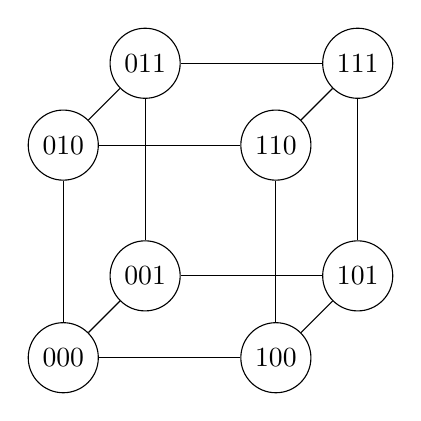
\begin{tikzpicture}[scale=0.9]
            \tikzstyle{myCir}=[circle,draw];
            \node[myCir] (000) at (0,0,0) {000};
            \node[myCir] (100) at (3,0,0) {100} edge (000);
            \node[myCir] (010) at (0,3,0) {010} edge (000);
            \node[myCir] (110) at (3,3,0) {110} edge (010) 
                                             edge (100);
            \node[myCir] (001) at (0,0,-3) {001} edge (000);
            \node[myCir] (101) at (3,0,-3) {101} edge (100) 
                                             edge (001);
            \node[myCir] (011) at (0,3,-3) {011} edge (010)   
                                             edge (001);
            \node[myCir] (111) at (3,3,-3) {111} edge (110) 
                                             edge (011) edge (101);
         \end{tikzpicture}
         & \hTwoOldd
         ${\displaystyle \quad\quad\quad
         \begin{matrix}
            \lvert V(\mathrm{Q}_{r})\rvert = 2^{r} \\ \\
            \lvert E(\mathrm{Q}_{r})\rvert = \frac{2^{r}r}{2} = 
               2^{r-1}r \\ \\ \\ \\{\teachCommentOldd\text{
                  Note that } \mathrm{Q}_{r} \text{ is } r
                  \text{-regular.}}
         \end{matrix}}$
      \end{tabular}
   \end{center}
\end{myIndent}

\newpage
\hOneOld
If $G=(V, E)$, then $H=(W, F)$ is a \udefine{subgraph} of $G$
if $W\subseteq V$ and $F\subseteq E$. \retTwo

If $W=V$, then $H$ is a \udefine{spanning subgraph} of $G$ (meaning 
that $H$ has the same vertices as $G$ but is lacking some of $G$'s 
edges) \retTwo

We define subtracting a set of vertices from a graph as follows:
\begin{myIndent} \hTwoOldd
   For $G = (V, E)$ and $X \subset V$, we define...
      \begin{myIndent}\begin{myIndent}
         ${\displaystyle G - X = (V \setminus X, \{\{u, v\}\in E 
         \mid \{u, v\}\cap X = \emptyset\}) }$
      \end{myIndent}\end{myIndent}
\end{myIndent}
\retTwo

\hOneOld % I might not actually need this command here...
We define subtracting a set of edges from a graph as follows:
\begin{myIndent} \hTwoOldd
   For $G = (V, E)$ and $L \subset E$, we define...
      \begin{myIndent}\begin{myIndent}\begin{myIndent}\begin{myIndent}
         ${\displaystyle G - L = (V, E \setminus L) }$
      \end{myIndent}\end{myIndent}\end{myIndent}\end{myIndent}
\end{myIndent} \retTwo

\hOneOld \markLecture{1/11/2024} \retTwo

We shall notate that $H$ is a subgraph of $G$ by 
writing $H \subseteq G$. \retTwo

An \udefine{induced subgraph} of $G = (V, E)$ is a subgraph 
$G\left[ X \right] = G - (V \setminus X)$ where $X \subseteq V$.
Alternatively, this is called the subgraph induced by $X$.
\retTwo

% Augh there is a bug with the uuline command I made!!!!
Given $G = (V, E)$ and $F \subseteq E$, the 
\udefine{subgraph spanned by $F$} is the subgraph whose edge set is $F$ 
and whose vertex set is ${\displaystyle
\bigcup_{e \in F}e}$. \retTwo

\mySepTwo \hOneOld
\begin{myIndent}\begin{myIndent}\begin{myIndent}\begin{myIndent}
   Here are some basic classes of graphs: \retTwo
\end{myIndent}\end{myIndent}\end{myIndent}\end{myIndent}

   \begin{itemize}
   \item \udefine{Complete graphs / cliques}, denoted $K_n$, are graphs 
      where every possible edge is present between $n$ vertices.\hTwoOldd

      \begin{center}
      \begin{allowTableDashes}\begin{tabular}
                           { c;{10pt/3pt}c;{10pt/3pt}c;{10pt/3pt}c c c }

         \begin{tikzpicture}[scale=0.5, inner sep=3pt]
            \useasboundingbox (-1.5,-3.5) rectangle (1.5,3);

            \tikzstyle{myCir}=[circle,fill];
            \node[myCir] (1) at (0:0) {};
            \node (name) at (270:3) {$K_1$};
         \end{tikzpicture}

         &

         \begin{tikzpicture}[scale=0.5, inner sep=3pt]
            \useasboundingbox (-3,-3.5) rectangle (3,3);

            \tikzstyle{myCir}=[circle,fill];
            \node[myCir] (1) at (0:2) {};
            \node[myCir] (2) at (180:2) {} edge (1);
            \node (name) at (270:3) {$K_2$};
         \end{tikzpicture}

         &

         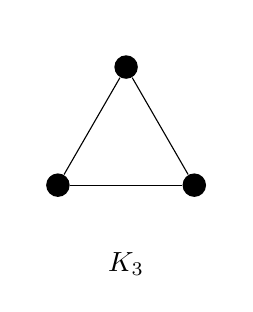
\begin{tikzpicture}[scale=0.5, inner sep=3pt]
            \useasboundingbox (-2.5,-3.5) rectangle (2.5,3);

            \tikzstyle{myCir}=[circle,fill];
            \node[myCir] (1) at (330:2) {};
            \node[myCir] (2) at (210:2) {} edge (1);
            \node[myCir] (3) at (90:2) {} edge (1) edge (2);
            \node (name) at (270:3) {$K_3$};
         \end{tikzpicture}

         &

         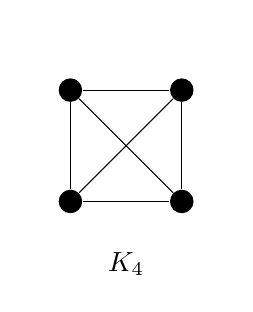
\begin{tikzpicture}[scale=0.5, inner sep=3pt]
            \useasboundingbox (-2.5,-3.5) rectangle (2.5,3);

            \tikzstyle{myCir}=[circle,fill];
            \node[myCir] (1) at (45:2) {};
            \node[myCir] (2) at (135:2) {} edge (1);
            \node[myCir] (3) at (225:2) {} edge (1) edge (2);
            \node[myCir] (4) at (315:2) {} edge (1) edge (2) edge (3);

            \node (name) at (270:3) {$K_4$};
         \end{tikzpicture}
      \end{tabular} \end{allowTableDashes}
      \end{center}

      
      \begin{myIndent}\begin{myIndent}\begin{myIndent}\begin{myIndent}
         \teachCommentOldd \begin{tabular}{ p{2.75in} c }
            
            Note we can also draw $K_4$ such that there are no edge
            interceptions as follows: &
         {\raisebox{-2.5em}{\tikz[scale=0.5, inner sep=3pt]{
            \tikzstyle{myCir}=[circle,fill];
            \node[myCir] (1) at (330:2) {};
            \node[myCir] (2) at (210:2) {} edge (1);
            \node[myCir] (3) at (90:2) {} edge (1) edge (2);
            \node[myCir] (4) at (0:0) {} edge (1) edge (2) edge (3);
         }}}
         \end{tabular}
      \end{myIndent}\end{myIndent}\end{myIndent}
      
      \hTwoOldd
      $\lvert V(K_n) \rvert = n$ \\
      $\lvert E(K_n) \rvert = \begin{pmatrix} n
         \vphantom{\frac{1}{1}} \\ 2\vphantom{\frac{
         \frac{1}{1}}{1}} \end{pmatrix} = \dfrac{n(n - 1)}{2}$ \retTwo
      \end{myIndent}
      \newpage

      \hOneOld
      \item A graph $G = (V, E)$ is bipartite if there exists a
         partition $(A, B)$ of $V$ such that every edge in $E$
         has one end in $A$ and one end in $B$. \retTwo
         {\hTwoOldd \begin{tabular}{p{2in} p{0.5in} p{3in}}
            \raisebox{-6em}{
               \tikz[scale=0.6, inner sep=3pt]{
                  \tikzstyle{myCir}=[circle, fill];

                  \draw[color=VioletRed, thick] 
                              (0, -1) arc (270:630:0.6 and 3);
                  \node (t) at (-1.25, 2) {{\color{VioletRed}\Huge A}};
                  
                  \draw[color=VioletRed, thick] 
                              (4, 0) arc (270:630:0.6 and 2);
                  \node (t) at (5.25, 2) {{\color{VioletRed}\Huge B}};
                  
                  \node[myCir] (t1) at (4,3) {};
                  \node[myCir] (t2) at (4,1) {};
                  \node[myCir] (s1) at (0,4) {} edge (t1) edge (t2);
                  \node[myCir] (s2) at (0,2) {} edge (t1);
                  \node[myCir] (s3) at (0,0) {} edge (t2); 
               }
            }
            &
            & 
            {The partition $(A, B)$ is called the \newline
            \udefine{bipartition} of $G$. Then $A$ and $B$ are called 
            the \udefine{parts} of $G$.}
         \end{tabular}} \retTwo

      \item A \udefine{Complete bipartite graphs} $K_{s,t}$, is the 
         bipartite graph with parts $A$ and $B$ where 
         $\lvert A \rvert = s$, $\lvert B \rvert = t$, and all 
         possible edges between $A$ and $B$ exist.

         \begin{myIndent}\begin{myIndent} \hTwoOldd
            For example, $K_{3,2}$: \hspace{2em} \raisebox{-2.3em}{
               \tikz[scale=0.5, inner sep=3pt]{
                  \tikzstyle{myCir}=[circle, fill];
                  \node[myCir] (t1) at (4,3) {};
                  \node[myCir] (t2) at (4,1) {};
                  \node[myCir] (s1) at (0,4) {} edge (t1) edge (t2);
                  \node[myCir] (s2) at (0,2) {} edge (t1) edge (t2);
                  \node[myCir] (s3) at (0,0) {} edge (t1) edge (t2); 
               }
            }
         \end{myIndent}\end{myIndent} \retTwo
   
      \item A \udefine{path} $P_k$ of length $k$ has a vertex set
         $V = \{v_1, v_2, \ldots, v_k, v_{k+1}\}$ and an edge set
         $E = \{\{v_1, v_2\}, \{v_2, v_3\}, \ldots, 
         \{v_{k-1}, v_k\}, \{v_k, v_{k+1}\}\}$.
      
         {\center \hTwoOldd
            Note that $\lvert V(P_k) \rvert = k+1$ and $\lvert E(P_k) 
            \rvert = k$. \\ Therefore, below would be $P_3$...
         
            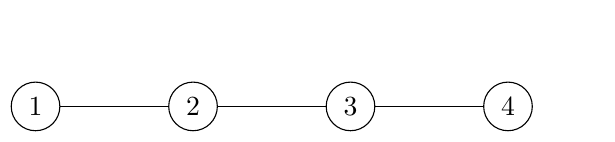
\begin{tikzpicture}
               \tikzstyle{myCir}=[circle, draw]

               \useasboundingbox (-0.1,-0.1) rectangle (7,1);

               \node[myCir] (4) at (6,0) {4};
               \node[myCir] (3) at (4,0) {3} edge (4);
               \node[myCir] (2) at (2,0) {2} edge (3);
               \node[myCir] (1) at (0,0) {1} edge (2);
            \end{tikzpicture} \retTwo
         
         \par }
      
      \item A \udefine{cycle} $C_k$ of length $k$ has a vertex set 
         $V = \{v_1, v_2, \ldots, v_k\}$ and an edge set $E = 
         \{\{v_1, v_2\}, \{v_2, v_3\}, \ldots, \{v_{k-1}, v_k\},
            \{v_k, v_1\}\}$.
         
         {\center \hTwoOldd
            Note that $\lvert V(C_k) \rvert = k$ and $\lvert E(C_k) 
            \rvert = k$. \\ Therefore, below would be $C_4$...

            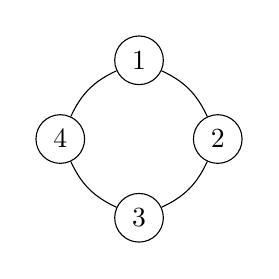
\begin{tikzpicture}[scale=0.5]
               \tikzstyle{myCir}=[circle, draw]

               \useasboundingbox (225:4) rectangle (45:4);

               \node[myCir] (2) at (0:2) {2};
               \node[myCir] (1) at (90:2) {1} edge [bend left=20] (2);
               \node[myCir] (4) at (180:2) {4} edge [bend left=20] (1);
               \node[myCir] (3) at (270:2) {3} edge [bend left=20] 
                        (4) edge [bend right=20] (2);
            \end{tikzpicture} \retTwo
         \par}

\end{itemize}
\newpage
Here is some terminology before the next lemma. For the graph
$G = (V, E)$\ldots
   
   \begin{itemize}
      \item $\delta(G) = \min\{d_G(v) \mid v \in V\}$ is the 
      \udefine{minimum degree} of $G$.
      \item $\Delta(G) = \max\{d_G(v) \mid v \in V\}$ is the 
      \udefine{maximum degree} of $G$.
      \item The \udefine{degree sequence} of $G$ is the 
      sequence of degrees of vertices $G$ in \\non-increasing order.
   \end{itemize}


\exOneOldd
\begin{center}
\begin{myClosureDeprecated}{5.5}
   \uuline{Lemma (part 1)}: If $G = (V, E)$ is a graph of minimum degree
   $k \geq 2$, then $G$ contains a cycle of length at least
   $k + 1$.

   {\exPOldd \begin{myConstrict}
      Proof: Let $P$ be a longest possible path in $G$, say:
      \[V(P) = \{v_1, v_2, \ldots, v_r\}\]

      Then $N(v_r) \subseteq V(P)$. After all, if this were not 
      the case, we'd be able to extend the path to the vertex in 
      $N(v_r)$ but not in $V(P)$, thus contradicting the fact that
      $P$ is a longest path. \retTwo

      Let $v_i$ be the first neighbor of $v_r$ along the path from
      $v_1$ to $v_r$. Then $\{v_i, v_{i+1}, \ldots, v_r\}$ are the
      vertices of a cycle $C$. \retTwo

      Now note that because $N(v_r) \subseteq P$ and $v_i$ was
      the first element in the path $P$ to belong to $N(v_r)$, 
      we know that $C$ contains all the elements of $P$ that 
      $N(v_r)$ also has. So, $N(v_r) \subseteq C$. \retTwo

      But now note that $\lvert N(v_r) \rvert \geq \delta(G)=k$. Plus,
      $v_r$ itself is not in $N(v_r)$. Combining these facts together,
      we can say that the cycle $C$ has at least $k + 1$ vertices.
   \end{myConstrict}}

   \uuline{Lemma (part 2)}: The cycle length $k+1$ is the longest 
   we can guarentee based on the minimum degree of the graph being $k$.

   {\exPOldd \begin{myConstrict}
      Proof: Take the graph $K_{k+1}$ which has a minimum degree $k$. 
      \newline
      Obviously, the longest cycle in $K_{k+1}$ is the cycle containing
      all $k+1$ elements of $K_{k+1}$. Thus, we have shown that there
      are graphs with minimum degree $k$ which don't have cycles of
      length greater than \newline $k + 1$.
   \end{myConstrict}} 
\end{myClosureDeprecated}
\end{center}
\retTwo

\hOneOld
A \udefine{connected graph} is a graph in which any two vertices
are the ends of a path. \retTwo

The \udefine{components} of a graph are the \uuline{maximal connected
subgraphs}. For example: \retTwo
{\hTwoOldd
   \begin{myIndent}\begin{myIndent}
      Let us define $G$ as: \hspace{2em}
      \raisebox{-2em}{\tikz[scale=0.4, inner sep=3pt]{
         \tikzstyle{myCir}=[circle, fill];
   
         \node[myCir] (t1) at (0, 1) {};
         \node[myCir] (t2) at (2, 1) {} edge (t1);
         \node[myCir] (t3) at (1, 3) {} edge (t1) edge (t2);
   
         \node[myCir] (y1) at (6, 2) {};
         \node[myCir] (y2) at (5, 4) {} edge (y1);
         \node[myCir] (y3) at (7, 4) {} edge (y1);
         \node[myCir] (y4) at (6, 0) {} edge (y1);
   
         \node[myCir] (p) at (10, 2) {};
   
         \draw[color=PineGreen, thick] 
                                 (-1.2, 2) arc (180:540:6 and 3);
      }} \retTwo

      As can be seen, $G$ has three components.
   \end{myIndent}\end{myIndent}
}
\newpage

A \udefine{tree} is a connected graph with no cycles
   (a.k.a it is acyclic). \hTwoOldd
   \begin{myIndent}
      Some examples of small trees include: $K_1$, $K_2$, $K_{1,2}$, 
      $P_3$, and $K_{1,3}$.
   \end{myIndent}

   \begin{center}
      \begin{myClosureDeprecated}{5.5}
         \uuline{Lemma}: Every tree with $n$ vertices has exactly
         $n - 1$ edges.
         \hThreeOld
         \begin{myConstrict}
            Proof: We shall proceed by induction. \retTwo
            
            If $n = 1$, the tree is $K_1$, meaning that it has $0=n-1$
            edges. \retTwo

            Now assume the lemma is true for all trees with $n$
            vertices, and let $T$ be a tree with $n+1$ vertices. Then,
            we shall remove a vertex $v$ of $T$ with degree $1$. 
            (Note that we know such a vertex must exist since 
            otherwise the minimum degree of $T$ would be 
            at least $2$ and that would guarentee a cycle exists 
            of at least length 3. This
            of course contradicts the fact that $T$ is acyclic.)
            \retTwo 
            Then $T - \{v\}$ is a tree with $n$ vertices as it must be acyclic and connected. 
            So by induction it has $n-1$ edges. And because
            $v$ has degree $1$, we know that \newline $\lvert E(T) \rvert
            = 1 + \lvert E(T - \{v\}) \rvert = 1 + (n - 1) = n$.
         \end{myConstrict} \retTwo
         \hTwoOldd

         \uuline{Lemma}: Any connected graph with finite vertices has a spanning tree.
         \hThreeOld
         \begin{myConstrict}
            Proof: \retTwo

            Firstly consider the case that the graph $G$ has no cycle.
            Then, it is a tree by definition. \retTwo

            Now, consider if $G$ has a cycle $C$. Then for any edge \newline
            $e \in E(C)$, we have that $G - \{e\}$ is still connected.
            So, we can now go back to the top of the proof and ask:
            does $G -\{e\}$ have any cycles? We can repeatedly do this
            until the graph has no cycles since taking away edges
            does not remove any vertices.
            
         \end{myConstrict}
         \teachCommentOldd
         \begin{myIndent}\begin{myIndent}
            \begin{myConstrict}
            This actually acts as an algorithm for finding a spanning
            tree of any connected graph.
            \end{myConstrict}
         \end{myIndent}\end{myIndent}
      \end{myClosureDeprecated}
   \end{center}\retTwo

\hOneOld

\begin{tabular}{ p{2in} p{1in} p{2.5in}}
   If $u$ and $v$ are two vertices in a connected graph, the
   \udefine{distance} from $u$ to $v$ is the length of a shortest
   path with ends at $u$ and $v$. & &
   \begin{centering} \hfill
      \raisebox{-6em}{\tikz[scale=0.9, inner sep=3pt, Black, very thick]{
            \tikzstyle{myCir}=[circle, fill];
            \tikzstyle{orng}=[color=Orange, line width=6pt, opacity=0.5];
      
            \node[myCir] (1) at (0, 0) {};
            \node[myCir] (2) at (2, 1) {} edge (1) edge[orng] (1);
            \node[myCir] (3) at (2, -1) {} edge (1) edge[orng] (1);
            \node[myCir] (4) at (3, 2) {} edge (2);
            \node[myCir, color=Red, label=above:{\color{red}$u$}] 
                  (5) at (4, .5) {} edge (2) edge[orng] (2);
            \node[myCir, color=Red, label=below:{\color{red}$v$}] 
                  (6) at (4, -.5) {} edge (3) edge[orng] (3);
            \node[myCir] (7) at (3, -2) {} edge (3);
            \node[myCir] (8) at (6, 1) {} edge (5);
            \node[myCir] (9) at (6, -1) {} edge (6);
         }}
   \end{centering}
\end{tabular}
\newpage

\hOneOld
Let $d_G(u, v)$ be the distance between $u$ and $v$.\retTwo

Distance is a \udefine{metric}, meaning:
\begin{myIndent}\begin{myIndent}\begin{enumerate}
   \item $d_G(u, v)=0 \Longleftrightarrow u=v$
   \item $d_G(u, v)=d_G(v, u)$
   \item $\forall w\in V, \hspace{0.5em}
      d_G(u, v) \leq d_G(u, w) + d_G(w, v)$
\end{enumerate}\end{myIndent}\end{myIndent} \retTwo

The \udefine{diameter} of a connected graph $G$ is the maximum distance
between any two vertices of $G$. Or in other words,
$\max\{d_G(u,v) \mid u,v\in  V(G)\}$. \retTwo

The \udefine{radius} of $G$ is equal to 
   $ \min\{\max\{d_g(u,v) \mid u\in V(G)\} \mid v\in V(G)\} $. What
   that means is that the radius of $G$ measures the smallest distance
   path one could limit themselves to drawing while still being able
   to have that path have one end at some fixed vertex and its other
   end at any arbitrary vertex in the graph.


\begin{myIndent}
   \hTwoOldd \uuline{Examples}:
   \begin{enumerate}
      \item The radius of $K_n$  is $1$. The diameter of $K_n$ is $n$.
      \retTwo
      \item The diameter of $P_k$ is $k$. The radius, can be computed as
         follows:
         \begin{myIndent} \hFourOldd
            The middle vertex of a path will have the fastest access
            to either end of the path. So, we shall measure the radius
            from the vertex: $v_{\lceil \frac{k+1}{2} \rceil}$. Then,
            we can see that $v_{k+1}$ is going to be a farthest element
            from $v_{\lceil \frac{k+1}{2} \rceil}$. So the radius
            of $P_k$ equals $k + \lceil \frac{k+1}{2} \rceil$.
            \retTwo

            Now you can consider what happens when $k$ is even and odd.
            But what's \\important is that it works out that the radius
            is $\lceil \frac{k}{2} \rceil$.
         \end{myIndent}
   \end{enumerate}
\end{myIndent} \retTwo
\hOneOld
We can use a \udefine{search tree} to more generally find
the radii and diameters of graphs. \retTwo

\begin{myIndent} \hTwoOldd
   \uuline{Breadth-First-Search}
   \begin{myIndent}
      Here's how to find a spanning tree in a connected graph with a root
      vertex $v$ such that the tree "preserves" all distances
      from $v$.
      (This tree is called a \udefine{BFS tree}).
      \begin{myIndent} \hThreeOld
         Let $G$ be a connected graph and let $(v_1, v_2, v_3,
         \ldots, v_n)$ be any ordering of the vertices of $G$.
         \retTwo
         Pick a vertex $v=v_1$ to be the root of the BFS tree.
         \retTwo
         Now, at any stage in constructing this tree, we will have
         a vertex set $V(T) = \{v_1, v_2 \ldots, v_k\}$ (when we first
         start, $V(T)$ will only contain $v_0$. So don't worry about that).
         Now if $V(T)=V(G)$ we can stop. Otherwise though, we can say 
         that there is a smallest integer $i$ such that for $v_i \in V(T)$, 
         $\hspace{0.25em} N(v_i)\setminus V(T) \neq \emptyset$.
         Choose $v_{k+1}$ to be the smallest neighbor (by the ordering of $V(G)$) of $v_i$ 
         not in $T$ and add 
         the edge $\{v_i, v_{k+1}\}$ to $T$. Then we repeat this paragraph.
         \retTwo
         Beware the ordering we are creating in our tree will often
         be different from the order of the graph you started with.
      \end{myIndent}
   \end{myIndent}
      \newpage
      \exOneOldd

      
   \begin{center}\begin{myClosureDeprecated}{5.5}
      \uuline{Worked Demonstration}: \retTwo
      \exTwoOldd
      \begin{tabular}{ c c c }
         \begin{centering}
            \raisebox{-5em}{\tikz[scale=0.45,inner sep=4pt]{
               \tikzstyle{myCir}=[circle, draw];

               \node[myCir] (9) at (18:2) {9};
               \node[myCir] (7) at (90:2) {7};
               \node[myCir] (8) at (162:2) {8}
                  edge (9);
               \node[myCir] (3) at (234:2) {3}
                  edge (9) edge(7);
               \node[myCir] (10) at (306:2) {10}
                  edge (7) edge(8);
               \node[myCir] (5) at (18:5) {5}
                  edge (9);
               \node[myCir] (6) at (90:5) {6}
                  edge (7) edge (5);
               \node[myCir] (2) at (162:5) {2}
                  edge (6) edge (8);
               \node[myCir] (1) at (234:5) {1}
                  edge (2) edge (3);
               \node[myCir] (4) at (306:5) {4}
                  edge (1) edge (10) edge (5);
            }\par}
         \end{centering}
         &
         becomes
         &
         \begin{centering}
            \raisebox{-5em}{\tikz[scale=0.45,inner sep=4pt]{
               \tikzstyle{myCir}=[circle, draw];

               \node[myCir] (9) at (18:2) {9};
               \node[myCir] (7) at (90:2) {7};
               \node[myCir] (8) at (162:2) {8};
               \node[myCir] (3) at (234:2) {3}
                  edge (7) edge (9);
               \node[myCir] (10) at (306:2) {10};
               \node[myCir] (5) at (18:5) {5};
               \node[myCir] (6) at (90:5) {6};
               \node[myCir] (2) at (162:5) {2}
                  edge (6) edge (8);
               \node[myCir] (1) at (234:5) {1} 
                  edge (2) edge (3);
               \node[myCir] (4) at (306:5) {4}
                  edge (1) edge (5) edge (10);
            }\par}
         \end{centering}
      \end{tabular}
   \end{myClosureDeprecated}\end{center} \retTwo

   \hTwoOldd
   \begin{myIndent}
      \uuline{Properties of BFS}: \hfill \bigbreak

      \begin{itemize}
         \item If the root is $v$, then $d_T(v, w) = d_G(v, w)$. In otherwords, a BFS tree \\preserves distances from its root. \newline
         
         \item The Tree with root $v$ has layers $N_i(v)=\{w\in V(G) \mid d_G(v, w)=i\}$. Furthermore all edges in the original graph either stay inside a single layer $N_i(v)$ or go between adjacent layers (i.e. from $N_i(v)$ to $N_{i+1}(v)$).
         {\begin{myIndent}\begin{myDindent}\begin{myDindent} \hThreeOld
            If an edge did "jump over" a layer, that \\violate the fact that distance is a metric. \newline
         \end{myDindent}\end{myDindent}\end{myIndent}}
         

         \item The diameter of $G$ equals the maximum number of
         layers of all BFS trees (not including the 0-layer). \newline

         \item The radius of $G$ equals the minimum number of layers
         of all BFS trees (also not including the 0-layer). \newline
      \end{itemize}
   \end{myIndent}
\end{myIndent}

\hOne
\mySepTwo \newline
\markLecture{1/16/2024}

Note that a tree is "minimally connecting" as subtracting any edge from a tree will produce a disconnected graph.
\begin{myIndent}
   We know this is the case because if we could remove an edge and still have the graph be connected, then that would imply the existence of a path between two neighboring vertices that doesn't go through their shared edge. But then, we'd be able to make a cycle subgraph by adding their shared edge to that path.
\end{myIndent}

\newpage

{\hTwo
\begin{myIndent}
   \uuline{Depth-First-Search}
   \begin{myIndent}
      Here is alternate algorithm for generating a spanning tree of a connected graph. A resulting tree of this algorithm is called a \udefine{DFS tree}.

      {\begin{myIndent} \hThree
         Let $G$ be a connected graph and let $(v_1, v_2, \ldots, v_n)$ be any ordering of the vertices of $G$. \retTwo

         Pick a vertex $v=v_1$ to be the root of the DFS-tree. \retTwo

         Now, at any stage in constructing this tree, we will have a vertex set $V(T)=\{v_1, v_2, \ldots, v_k\}$. If $V(T)=V(G)$, we can stop. Otherwise though, we select $i$ to be the largest integer such that for $v_i \in V(T)$,\\ $\hspace{0.25em} N(v_i)\setminus V(T) \neq \emptyset$. Then, choose $v_{k+1}$ to be the smallest neighbor (by the ordering of $V(G)$) of $v_i$ not in $V(T)$ and add 
         the edge $\{v_i, v_{k+1}\}$ to $T$. Then we repeat this paragraph.
         \retTwo
         Once again beware the ordering we are creating in our tree will typically be different from the order of the graph you started with. \retTwo
      \end{myIndent}}
   \end{myIndent}

   {\exOne
   \begin{center}\begin{myClosureDeprecated}{5.5}
      \uuline{Worked Demonstration}: \retTwo
      \exTwoOldd
      \begin{tabular}{ c c c }
         \begin{centering}
            \raisebox{-5em}{\tikz[scale=0.45,inner sep=4pt]{
               \tikzstyle{myCir}=[circle, draw];

               \node[myCir] (3) at (4,2) {3};
               \node[myCir] (2) at (-4,2) {2}
                  edge (3);
               \node[myCir] (1) at (-4,-2) {1}
                  edge (2) edge (3);
               \node[myCir] (4) at (4,-2) {4}
                  edge (3) edge (2) edge (1);
               \node[myCir] (5) at (0,5) {5}
                  edge (2) edge (3);
               \node[myCir] (6) at (0,-5) {6}
                  edge (1) edge (4);
            }\par}
         \end{centering}
         &
         becomes
         &
         \begin{centering}
            \raisebox{-5em}{\tikz[scale=0.45,inner sep=4pt]{
               \tikzstyle{myCir}=[circle, draw];

               \node[myCir] (3) at (4,2) {3};
               \node[myCir] (2) at (-4,2) {2}
                  edge (3);
               \node[myCir] (1) at (-4,-2) {1}
                  edge (2);
               \node[myCir] (4) at (4,-2) {4}
                  edge (3);
               \node[myCir] (5) at (0,5) {5}
                  edge (3);
               \node[myCir] (6) at (0,-5) {6}
                  edge (4);
            }\par}
         \end{centering}
      \end{tabular}
   \end{myClosureDeprecated}\end{center}} \hTwo\retTwo

   \mySepTwo[Black]

   \uuline{Theorem}: A graph is bipartite if and only if it contains no odd cycles.

   {\hThree
   \begin{myIndent}
      Proof: \\($\Longrightarrow$) First note that an odd cycle isn't bipartite. Thus, any graph containing an odd cycle is not bipartite. \retTwo

      ($\Longleftarrow$) Now supposed we are given some graph $G$ with no odd cycles. \\
      Then, assuming $G$ is connected (if $G$ isn't connected, we can break $G$ up into its component subgraphs and do this process for each component), we can construct a BFS-tree in $G$ rooted at some $v\in V(G)$. Let us name this tree $T$.
      \newpage

      Now as noted before, $T$ will have layers $L_i$ where each \\ $L_i=\{u\in V(G) \mid d_G(v, u)=i\}$. Using those layers, we can partition $T$ into two subsets $A$ and $B$ where $A$ is the union of all $L_i$ where $i$ is even and $B$ is the union of all $L_j$ where $j$ is odd. So, $T$ is clearly bipartite.
      \retTwo

      Now, let's reinsert the removed edges from $G$ back into $T$. Note that for each re-inserted edge $e$, it must be the case that either $e$ is a subset of some $L_i$ or that $e$ goes between some $L_i$ and $L_{i+1}$. Importantly, edges of the latter case do not violate our partition. So, if all the edges in $E(G) \setminus E(T)$ go between layers, then we can conclude that $G$ is definitely bipartite just like $T$.
      \retTwo

      With that, we now intend to show that an edge $G$ having an edge belonging to a single layer $L_i$ guarentees that $G$ contains an odd cycle.
      {\begin{myIndent} \hFour
         Assume the graph $G$ has an edge $\{u, w\}\subseteq L_i$ where $L_i$ is the $i$th layer of a BFS tree rooted at $v$. Then, we know that there exists a path $P_1$ contained in that BFS tree going from $v$ to $u$ and a path $P_2$ contained in that BFS tree going from $v$ to $w$. In order to draw a cycle from this information, let $x$ be the vertex of some $L_j$ such that $x\in V(P_1)$, $x\in V(P_2)$, and $j$ is as large as possible. That way, by defining the subpaths ${P_1}^\prime$ going from $x$ to $u$ and ${P_2}^\prime$ going from $x$ to $w$, we can get the following cyclic subgraph of $G$ :\[ C=(V({P_1}^\prime)\cup V({P_2}^\prime), E({P_1}^\prime)\cup E({P_2}^\prime) \cup \{u, w\})\]

         However, now note that $\lvert E({P_1}^\prime) \rvert = \lvert E({P_2}^\prime) \rvert = i-j$. Hence, \\$\lvert E(C) \rvert = 2(i-j)+1$, which in turn means that $C$ has an odd number of edges. So, we have shown that if a graph $G$ contains an edge within a single layer $L_i$, then we can give an example of an odd cycle within $G$. \retTwo
      \end{myIndent}}

      So in conclusion, if we assume $G$ has no odd cycles, then $G$ can't have any edges which are subsets of a single layer $L_i$. But that means that every edge in $G$ respects the partition we made to show that $T$ is bipartite. So, $G$ must also be bipartite with the same partition as $T$. $\blacksquare$
   \end{myIndent}
   }
\end{myIndent}}

\hOne
\mySepOne

A \udefine{Hamiltonian cycle} is a spanning cycle of a graph. We say a graph is \udefine{Hamiltonian} if it contains such a cycle. \retTwo

A \udefine{Hamiltonian path} is a spanning path of a graph. We say a graph is \udefine{traceable} if it has a hamiltonian path. \retTwo

A \udefine{walk} is a sequence of vertices and edges: i.e. $(v_1, \{v_1, v_2\}, v_2, \{v_2, v_3\}, ...)$

{\begin{myTindent} \teachComment
   Note that a walk can go over the same edge or vertex multiple times. \retTwo
\end{myTindent}}

A \udefine{trail} is a walk with no repeated edge.
{\begin{myTindent} \teachComment
   Interestingly, all paths are trails and all trails are walks. So a trail is kind of a middle concept between being a walk or a path.\retTwo
\end{myTindent}}
\newpage
A \udefine{tour} is a trail with the same first and last vertex.
{\begin{myTindent} \teachComment
   So, all cycles are tours and all tours are walks.\retTwo
\end{myTindent}}

An \udefine{Eulerian tour} of a graph is a tour which contains all the edges of the graph.
{\begin{myIndent} \hTwo
   For context, the name Eulerian is in honor of Leonhard Euler because he was the first mathematician to ask when a graph would have an Eulerian tour (look up the Seven Bridges of Königsburg problem). \retTwo
\end{myIndent}}

We call a graph \udefine{Eulerian} if for every vertex $v$ in the graph: $d(v)$ is even.

\mySepTwo

\markLecture{1/18/2024}

Before finding conditions for the existence of an eulerian tour of a graph, let's \\establish some terminology for digraphs so that we can study Eulerian tours in \\digraphs as well. \retTwo

Firstly, a walk, trail, and tour are defined almost identically in a digraph as in a graph. The one difference is that given some edge $(u, v)$ of a digraph, a walk, trail, and path are only allowed to traverse that edge going from $u$ to $v$. \retTwo

Given a digraph $(V, E)$, the "out" and "in" neighborhoods of a vertex $v \in V$ are:
\begin{myIndent}
   \begin{itemize}
      \item[{\color{BrickRed}out:}] $N^+(v)=\{w\in V \mid (v, w) \in E\}$
      \item[{\color{BrickRed}\phantom{o}in:}] $N^-(v)=\{w\in V \mid (w, v) \in E\}$
   \end{itemize}
\end{myIndent} \retTwo

Similarly, the out-degree and in-degree of $v \in V$ are:
\begin{myIndent}
   \begin{itemize}
      \item[{\color{BrickRed}out:}] $d^+(v)=\lvert N^+(v) \rvert$
      \item[{\color{BrickRed}\phantom{o}in:}] $d^-(v)=\lvert N^-(v) \rvert$
   \end{itemize}
\end{myIndent} \retTwo

A digraph is called \udefine{Eulerian} if for each vertex $v \hspace{0.25em}$, $d^+(v)=d^-(v)$.
{\center \exOne
   \begin{tabular}{ p{1.5in} p{3in} }
      \raisebox{-5em}{\tikz[scale=0.45,inner sep=3pt]{
         \tikzstyle{myCir}=[circle, draw, thick, color=Purple];
         \tikzstyle{inEdge} = [thick, color=Purple, arrows = {Stealth[scale=1.5]-}];
         \tikzstyle{outEdge} = [thick, color=Purple, arrows = {-Stealth[scale=1.5]}];
   
         \node[myCir] (1) at (0, 0) {$v_1$};
         \node[myCir] (3) at (5, 0) {$v_3$}
            edge [outEdge] (1);
         \node[myCir] (2) at (2.5, 4) {$v_2$}
            edge [inEdge] (1)
            edge [inEdge] (3);
      }}
      &
      \[{\begin{matrix}
         & d^+(v_1) = 1 & & d^+(v_2) = 0 & & d^+(v_3) = 2 \\
         & d^-(v_1) = 1 & & d^-(v_2) = 2 & & d^-(v_3) = 0
      \end{matrix}}\]
      This digraph is not Eulerian.
   \end{tabular}
\par} \retTwo

An \udefine{orientation} of a graph $G$ is a digraph with the same vertices as $G$ but where each $\{u, v\} \in E(G)$ is replaced with either $(u, v)$ or $(v, u)$. \retTwo

The \udefine{underlying graph} (or multigraph) of a digraph $G$ is the graph (or multigraph) such that $\{u, v\}$ is an edge whenever $(u, v) \in G$.
\newpage

{\begin{myIndent} \hTwo
   \uuline{Theorem}: 
   \begin{enumerate}
      \item A graph has an Eulerian tour if and only if it is connected and Eulerian.
      \item A digraph has an Eulerian tour if and only if it has a connected underlying graph and if it is Eulerian. \retTwo
   \end{enumerate}

   \hThree
   Proof of statement 1:
   \begin{myIndent}
      ($\Longrightarrow$) If $G$ has an Eulerian tour $v_0 e_0 v_1 e_1 v_2 e_2 \ldots v_k e_k v_0$, then for any $v_i$, the tour has to use an edge into $v_i$ and an edge out of $v_i$ each time it visits $v_i$. So, $d(v_i)$ is even for all $i$. \retTwo

      ($\Longleftarrow$) Now suppose $G$ is connected and all vertices have even degree. Then let $T=v_0 e_0 v_1 e_1 v_2 e_2 \ldots v_l e_l v_{l+1}$ be a longest trail in $G$. \retTwo
      
      If $v_{l+1} \neq v_0$, then we know that $v_{l+1}$ has an odd degree in $T$ as the trail goes into $v_{l+1}$ and doesn't leave. However, because we assumed that all vertices in $G$ have an even degree, we know there must be an even number of edges coming out of $v_{l+1}$. So, we can add another edge to our trail to get a longer trail. But this contradicts our assumption that $T$ is a longest trail in $G$. Hence, we conclude that $v_{l+1} = v_0$, meaning $T$ is a tour.\retTwo
      
      Now consider if $T$ is not an Eulerian tour. In that case, there is an edge of $G$ not in $T$. Additionally, because $G$ is connected, we know that that edge will have the form $e = \{v_i, w\}$. So now consider a new trail: $T^\prime$ defined as $v_i e_i v_{i+1} e_{i+1} \ldots v_0 e_0 v_1 e_1 \ldots v_i e w$. Importantly, $T^\prime$ is a longer trail than $T$. So we have a contradiction as $T$ is not a longest trail. \retTwo

      Therefore, the longest trail $T$ in $G$ must be an Eulerian tour. \retTwo
   \end{myIndent}

   The proof of statement 2 is nearly identical. \retTwo
   
   {\center \teachComment
   \begin{myClosureDeprecated}{4.5}
      Note that this proof can be interpretted as giving an algorithm for finding an Eulerian tour.
      \begin{enumerate}
         \item Make a trail $T$.
         \item Add edges to $T$ until you get stuck at a vertex. Then you know that your trail forms a tour.
         \item If $T$ is not an Eulerian tour, then going by the steps in the proof above, define $T^\prime$. Then do step 2. on $T^\prime$.
         \item If $T$ is an Eulerian tour, you're done.
      \end{enumerate}\end{myClosureDeprecated}\par}
\end{myIndent}}

\newpage

A harder problem is whether a graph has a Hamiltonian (spanning) cycle or not. \retTwo


{\exOne\begin{center}
   \begin{myClosureDeprecated}{5}
         {\exTwo \begin{tabular}{ p{2in} p{2.5in} }
         This graph \uuline{does not} have a Hamiltonian cycle.
         &
         \begin{centering}
            \raisebox{-5em}{\tikz[scale=0.45,inner sep=3pt]{
               \tikzstyle{myCir}=[circle, fill];
         
               \node[myCir] (9) at (18:2) {};
               \node[myCir] (7) at (90:2) {};
               \node[myCir] (8) at (162:2) {}
                  edge (9);
               \node[myCir] (3) at (234:2) {}
                  edge (9) edge(7);
               \node[myCir] (10) at (306:2) {}
                  edge (7) edge(8);
               \node[myCir] (5) at (18:5) {}
                  edge (9);
               \node[myCir] (6) at (90:5) {}
                  edge (7) edge (5);
               \node[myCir] (2) at (162:5) {}
                  edge (6) edge (8);
               \node[myCir] (1) at (234:5) {}
                  edge (2) edge (3);
               \node[myCir] (4) at (306:5) {}
                  edge (1) edge (10) edge (5);
            }}\par
         \end{centering}
         \\ & \\
         This graph \uuline{does} have a \newline Hamiltonian cycle.
         &
         \begin{centering}
            \raisebox{-5em}{\tikz[scale=0.45,inner sep=3pt]{
               \tikzstyle{myCir}=[circle, fill];
      
               \node[myCir] (0) at (0:0) {};
               \node[myCir] (1) at (18:4) {}
                  edge (0);
               \node[myCir] (2) at (90:4) {}
                  edge (1) edge (0);
               \node[myCir] (3) at (162:4) {}
                  edge (2) edge (0);
               \node[myCir] (4) at (234:4) {}
                  edge (3) edge (0);
               \node[myCir] (5) at (306:4) {}
                  edge (1) edge (4) edge (0);
            }}\par
         \end{centering}
      \end{tabular}}
   \end{myClosureDeprecated}
\end{center}} \retTwo

{\hTwo
\begin{myIndent}
   \uuline{Dirac's Theorem}: Let $n \geq 3$ and let $G$ be an $n$-vertex graph of minimum degree at least $\frac{n}{2}$. Then $G$ is hamiltonian. \retTwo

   
   {\begin{myIndent} \hThree
      Proof:\\ Suppose the theorem is false. Let $G$ be a counter-example with as many edges as possible (a maximal counter-example). Then, we know there exists an edge $\{u, v\} \notin E(G)$ as $G$ cannot equal $K_n$ since $K_n$ is hamiltonian. Furthermore, we know that $G + \{u, v\}$ is hamiltonian since $G$ was maximal. So, there is a hamiltonian cycle $C \subseteq G + \{u, v\}$ using the edge $\{u, v\}$. This in  turn means that $C - \{u, v\}$ is a hamiltonian path belonging to $G$.
      \retTwo

      Let $P=v_1e_1v_2e_2\ldots e_nv_n$ be the hamiltonian path in $G$ from $u$ to $v$ and let $N^+(w)$ denote the set of vertices immediately following a neighbor of $w$ on the path $P$. In other words: $N^+(w) = \{v_{i+1} \mid v_i \in N_G(w)\}$. \retTwo

      By the theorem's assumption about the minimum degree of the graph,\\ we know that $\left| N_G(u) \right| \geq \frac{n}{2}$. Meanwhile on the other end of $P$, since\\ $v=v_n \notin N_G(v)$, we know that every neighbor of $v$ has an element\\ following it on the path. So $\left| N^+(v) \right| \geq \frac{n}{2}$. Thus $\left| N_G(u) \right| + \left| N^+(v) \right| \geq n$.\\ But now note that $u$ does not belong to either of the above sets. So\\ $\left| N_G(u) \cup N^+(v) \right| \leq n-1$. As a consequence of this, $\left| N_G(u) \cap N^+(v) \right| > 0$. 
      
      \newpage

      Let $v_i$ be a vertex belonging to $(N_G(v) \cap N^+(u))$. Then we can draw a cycle in $G$ visiting all the vertices of $G$ in the following order: \[v_1, v_2, \ldots, v_{i-1}, v_n, v_{n-1}, \ldots, v_i, v_1\]

      This contradicts our assumption that $G$ would be a counter example and thus not Hamiltonian. So, we assume no such counter example exists. \retTwo
   \end{myIndent}}

   We can also show that Dirac's Theorem gives the best possible minimum degree for a graph to be guarenteably Hamiltonian. Consider a graph $G$ containing two copies of $K_m$ sharing exactly one vertex. In that case, $n = \left| V(G) \right| = 2m - 1$ and\\ $\delta(G) = m-1 = \frac{n-1}{2}$. However, this graph does not have a spanning subcycle as any spanning cycle would have to cross that shared vertex twice. \retTwo
\end{myIndent}}

\mySepTwo

Let $P$ be a longest path in $G$ going from a vertex $u$ to a vertex $v$. Additionally, for any $w \in V(P)$, let $w^+$ be the vertex following $w$ as one travels from $u$ to $v$ along $P$. Importantly, since $P$ is a longest path, we know that $(N_G(u) \cup N_G(v)) \subseteq V(P)$. Furthermore, for each $w \in N_G(v)$, we can define $Q = P - \{w, w^+\} + \{v, w\}$ where $Q$ is a longest path of $G$ going from $u$ to $w^+$ instead of $u$ to $v$. We call $Q$ a \udefine{rotation} of $P$ at $v$.
\retTwo

{\begin{myIndent} \hTwo
   \uuline{Pósa's Rotation Lemma}: Suppose $G$ is a graph and for every $S \subseteq V(G)$ with $\left| S \right| \leq t$, $\left| N(S) \right| > 2 \left| S \right|$. Then $G$ contains a path of length $3t + 1$.
   {\begin{myTindent} \hFour
      $N(S)$ is referring to the union of the neighborhoods of each $v \in S$ minus any vertices in $S$.
   \end{myTindent}}
   \retTwo
   
   {\begin{myIndent} \hThree
      Proof:\\ Let $P$ be a longest path ending at a vertex $v$. Also, let $S$ be the set of end \\vertices of all possible longest paths that could be obtained through any \\number of rotations starting with $P$. Finally, let $S^+$ and $S^-$ denoted the \\vertices of $P$ immediately after and immediately before vertices in $S$ \\respectively. \retTwo

      Obviously, $\lvert S^+ \rvert \leq \lvert S \rvert$ and $\lvert S^- \rvert \leq \lvert S \rvert$ as all vertices except the first and last vertex of $P$ have exactly one vertex before and after them in $P$. Also note that $N(S) \subseteq S^+ \cup S^-$. This is because if there did exist $w \in N(S)$ such that $w \notin S^+ \cup S^-$, then we would know that no rotation of $P$ made it so that $w$ was not proceeded by $w^-$ and followed by $w^+$. So, doing a rotation with the vertex $w$, we would show that either $w^+$ or $w^-$ belonged to $S$, thus reaching a contradiction. 
      \newpage

      Overall, this means that $\lvert N(S) \rvert \leq \lvert S^+ \cup S^- \rvert \leq \lvert S^+ \rvert + \lvert S^- \rvert \leq 2 \lvert S \rvert$.\\ However, note that by the theorem's assumption about $G$, we know that $\left|S\right| \geq t$ because otherwise we'd have that $ 2\left| S \right| < \left|N(S)\right|$. So, let $T$ be a subset of $S$ such that $\left| T \right| = t$. Then, because $T$ and $N(T)$ are disjoint\\ subsets of $(S \cup N(S))$ which itself is a subset of $V(P)$, we know that\\ $\left| V(P) \right| \geq \left| T \right| + \left| N(T) \right|$. And since $\left| N(T) \right| > 2\left| T \right| = 2t$ by the theorem's assumption about $G$, we thus can say that $\left| V(P) \right| > 3t$. $\blacksquare$ \retTwo
   \end{myIndent}}
\end{myIndent}}

\markLecture{1/23/2024}

{\begin{myIndent} \hTwo
   \uuline{Theorem}: If for every set $S$ of vertices in a graph $G$, we have that\\ $\left| N(S) \right| \geq \min{\{2\left|S\right| + 1, \hspace{0.25em} \left|V(G) \setminus S \right|\}}$, then $G$ has a hamiltonian path. \retTwo

   {\begin{myIndent} \hThree
      Proof:\\ Once again let us define $P$ as a longest path of $G$, as well as $S$ as the set of end vertices of all possible rotations of $P$. Then by the same reasoning as before, we know that $\left| N(S) \right| \leq 2 \left| S \right|$. Therefore, since $\left| N(S) \right|$ isn't greater than or equal to $2 \left| S \right| + 1$, we know by the assumption of the theorem that $N(S)$ is greater than or equal to $\left|V(G) \setminus S \right|$. \retTwo

      Now $S \cup (V(G) \setminus S) = V(G)$ and $(S \cup N(S)) \subseteq V(P)$. Additionally, $S$ and $(V(G) \setminus S)$ are disjoint to each other, as is $S$ and $N(S)$. Thus, we can say that \[
         \left| V(G) \right| = \left| S \right| + \left| (V(G) \setminus S) \right| \geq \left| S \right| + \left| N(S) \right| \leq \left| V(P) \right| \]
      
      Therefore the longest path $P$ must cover every vertex of $G$, meaning that it is a Hamiltonian path. $\blacksquare$\retTwo
      {\begin{myTindent} \teachComment
         This is what is used to find Hamiltonian paths in random graphs.
      \end{myTindent}}
   \end{myIndent}}
\end{myIndent}}

\mySepTwo

A graph is \udefine{uniquely Hamiltonian} if it has exactly one Hamiltonian cycle. \retTwo

{\begin{myIndent} \hTwo
   \uuline{Theorem}: If all vertices in a graph $G$ have odd degree, then every edge is in an even number of hamiltonian cycles.
   
   {\begin{myTindent}\begin{myIndent} \teachComment
      In other words such a graph is not uniquely Hamiltonian. \retTwo
   \end{myIndent}\end{myTindent}}
   {\begin{myIndent} \hThree
      Proof: \\
      If the graph $G$ in the theorem has no hamiltonian cycles, then we're done. Every edge is in $0$ hamiltonian cycles. \retTwo

      Now pick an edge and suppose that there is a Hamiltonian cycle $C$ containing it. We'll call that edge $\{u, v\}$ and let $w$ be the vertex coming before $u$ on $C$. \retTwo
      
      Then, let us define a new graph $H$ whose vertices are Hamiltonian paths in $G$ which start with the edge $\{u, v\}$. For example, $(C - \{u, w\}) \in V(H)$. Additionally, let $\{P, Q\}$ be an edge of $H$ if $P$ and $Q$ are rotations of each other. \retTwo

      If $P \in V(H)$ is a hamiltonian path in $G$ ending in a vertex $x \in V(G)$, then: \[d_H(P) = \left\{\begin{matrix}
         d_G(x) - 1 & & x \notin N_G(u) \\
         d_G(x) - 2 & & x \in N_G(u)
      \end{matrix}\right.\]
      {\begin{myIndent} \hFour
         Essentially, for every edge connecting to $x$ except for the one already used by $P$, there is a rotation of $P$. We can then say that that rotation is a vertex of $H$ if it includes the edge $\{u, v\}$ (In other words, a rotation including the edge $\{u, x\}$ would not be included in $H$).
      \end{myIndent}}

      \retTwo
      If $x$ is adjacent to $u$, then $P + \{\{u, x\}\}$ is a hamiltonian cycle containing $\{u, v\}$. \retTwo

      Now here is the clever part: since $d_G(x)$ is assumed to be odd for all \\$v \in V(G)$, we have that $d_H(P)$ is even if $x$ is not adjacent to $u$ and odd if $x$ is adjacent to $u$. But now note that every graph has an even number of vertices of odd degree because of the handshaking lemma. So, there must be an even number of paths including the edge $\{u, v\}$ and ending in a vertex $x$ such that $x$ is adjacent to $u$. Or in other words, $G$ has an even number of hamiltonian cyles containing the edge $\{u, v\}$. $\blacksquare$
   \end{myIndent}}
\end{myIndent}} \retTwo

{\exOne \center
   \begin{myClosureDeprecated}{5.2}
      For example, by the above theorem we know that this graph is not uniquely Hamiltonian.
      {\exTwo\center\raisebox{0em}{\tikz[scale=0.25,inner sep=3pt]{
         \tikzstyle{myCir}=[circle, fill, thick, color=RedViolet];
         \tikzstyle{myLine}=[thick, color=RedViolet];
   
         \node[myCir] (0) at (90.0:8) {};
         \node[myCir] (1) at (115.0:8) {}
               edge[myLine] (0);
         \node[myCir] (2) at (141.0:8) {}
               edge[myLine] (1);
         \node[myCir] (3) at (167.0:8) {}
               edge[myLine] (2);
         \node[myCir] (4) at (192.0:8) {}
               edge[myLine] (3);
         \node[myCir] (5) at (218.0:8) {}
               edge[myLine] (4);
         \node[myCir] (6) at (244.0:8) {}
               edge[myLine] (5) edge[myLine] (1);
         \node[myCir] (7) at (270.0:8) {}
               edge[myLine] (6) edge[myLine] (3);
         \node[myCir] (8) at (295.0:8) {}
               edge[myLine] (7) edge[myLine] (4);
         \node[myCir] (9) at (321.0:8) {}
               edge[myLine] (8);
         \node[myCir] (10) at (347.0:8) {}
               edge[myLine] (9) edge[myLine] (0);
         \node[myCir] (11) at (372.0:8) {}
               edge[myLine] (10) edge[myLine] (2);
         \node[myCir] (12) at (398.0:8) {}
               edge[myLine] (11) edge[myLine] (9);
         \node[myCir] (13) at (424.0:8) {}
               edge[myLine] (12) edge[myLine] (0) edge[myLine] (5);
      }}\par}
      One note about the above theorem is that it can be interpretted as giving an algorithm for finding a second hamiltonian cycle given one hamiltonian cycle in a graph where all degrees are odd.
   \end{myClosureDeprecated}
\par}

\newpage

A \udefine{matching} in a graph is a set of vertex disjoint edges in the graph. \retTwo

A vertex is \udefine{saturated} by a matching if one of the edges of the matching contains the vertex. Otherwise, we say the vertex is \udefine{exposed} by the matching. \retTwo

{\begin{center} \exOne
   \begin{tabular}{ p{3in} p{3in} }
      \\
         {\center\raisebox{0em}{\tikz[scale=0.35,inner sep=3pt]{
         \tikzstyle{myCir}=[circle, fill, thick];
         \tikzstyle{myLine}=[thick];
         \tikzstyle{myHL}=[color=Orange, line width=8pt, opacity=0.25];
         \useasboundingbox (-5,-5) rectangle (5, 2);
   
         \node[myCir, label=above:1] (0) at (90.0:5) {};
         \node[myCir, label=above:2] (1) at (141.0:5) {}
               edge[myLine] (0) edge[myHL] (0);
         \node[myCir, label=left:3] (2) at (192.0:5) {}
               edge[myLine] (1);
         \node[myCir, label=below:4] (3) at (244.0:5) {}
               edge[myLine] (2) edge[myHL] (2);
         \node[myCir, label=below:5] (4) at (295.0:5) {}
               edge[myLine] (3);
         \node[myCir, label=right:6] (5) at (347.0:5) {}
               edge[myLine] (4) edge[myHL] (4);
         \node[myCir, label=above:7] (6) at (398.0:5) {}
               edge[myLine] (5) edge[myLine] (0);
      }}\par} &
      The matching shown to the left is: \newline
      $M = \{\{1, 2\}, \{3, 4\}, \{5, 6\}\}$ \retTwo
      In the matching to the left, $7$ is \newline exposed and all other vertices are \newline saturated.
   \end{tabular}
\end{center}}

A \udefine{maximum matching} in a graph is a matching with the maximum number of edges. \retTwo

A \udefine{perfect matching} (or $1$-factor) is a matching which saturates all the vertices of a graph.
{\begin{myTindent}\begin{myTindent} \teachComment
   Proposition: for a graph to have a perfect matching, it must have an even number of vertices. 
\end{myTindent}\end{myTindent}}
\retTwo

\markLecture{1/30/2024}

{\begin{myIndent} \hTwo
   \uuline{Hall's Theorem}: Let $G$ be a bipartite graph with parts $A$ and $B$. Then $G$ has a \\matching saturating $A$ if and only if for every set $X \subseteq A$, \[ \lvert N_G(X) \rvert \geq \lvert X \rvert\text{.}\]
   {\begin{myTindent}\begin{myIndent} \teachComment
      Note: we refer to the below statement as \uuline{Hall's condition}: 
      \begin{myConstrict}\begin{myConstrict}
         $\forall X \subseteq A, \hspace{0.4em} \lvert N_G(X) \rvert \geq \lvert X \rvert$. \retTwo
      \end{myConstrict}\end{myConstrict}
   \end{myIndent}\end{myTindent}}

   {\begin{myIndent} \hThree
      Proof:\\
      ($\Longrightarrow$) If $G$ has a matching $M$ containing $A$, then for any $X \subseteq A$, we trivially have that $\left| N_G(X)\right| \geq \left| N_m(X) \right| = \left| X \right|$. \retTwo
      ($\Longleftarrow$) To prove the other way, we proceed by induction on $A$ while assuming Hall's condition is true. \retTwo

      Base case: assume that $\left| A \right| = 1$. In that case, because Hall's condition is assumed to be true, we know that $\left| N_G(A) \right| \geq \left| A \right| = 1$. Thus, for some $a \in A$ and $b \in B$, we know there exists an edge $\{a, b\} \in E(G)$. The matching of just that edge saturates $A$.

      \newpage

      Induction step:  Assume that Hall's theorem works if $1 \leq \left| A \right| < n$. Then assume that $\left| A \right| = n$. Since we are assuming Hall's condition to be true, we know that for all proper subsets $X \subset A$, either $\lvert N_G(X) \rvert > \lvert X \rvert$ or\\ $\lvert N_G(X) \rvert = \lvert X \rvert$ is true. \retTwo

      \begin{itemize}
         \item Case 1: For all proper subsets $X$ of $A, \hspace{0.5em}\lvert N_G(X) \rvert > \lvert X \rvert$\dots\\ {\hFour
            Pick an edge $\{a, b\} \in E(G)$ and consider $H = G - \{a\} - \{b\}$. We know that $H$ will be a bipartite graph with two sets of vertices: $A^\prime = A \setminus \{a\}$,\\ and $B^\prime = B \setminus \{b\}$. Additionally, given any $X \subseteq A^\prime$, we know that\\ $\lvert N_H(X) \rvert \geq \lvert N_G(X) \rvert - 1 \geq \lvert X \rvert$. So, by our inductive hypothesis, $H$ has a matching covering $A^\prime$. Now add the edge $\{a, b\}$ to this matching to get a matching in $G$ covering $A$.
         } 
         \retTwo

         \item Case 2: There exists a proper subset $X$ of $A$ such that $\left|N_G(X)\right| = \left| X \right|$\dots\\ {\hFour
            In this second case our reasoning for case 1 breaks down because given $X \subseteq A^\prime$, we can no longer guarentee that $\lvert N_G(X) \rvert - 1 \geq \lvert X \rvert$. So, using that same set $X$,  consider $G_1$ the induced graph of $N_G(X) \cup X$ and $G_2$ equal to $G - V(G_1)$. \retTwo

            For any $Y \subseteq X$, we have that $\left| N_{G_1}(Y) \right| = \left| N_G(Y) \right| \geq \left| Y \right|$ due to Hall's\\ condition. Thus, by our inductive hypothesis there exists a matching $M_1$ saturating $X$ in $G_1$. \retTwo

            Additionally, for any $Y \subseteq A \setminus X$, consider $N_G(Y \cup X)$. By assuming Hall's condition, we know that $\lvert N_G(Y \cup X) \rvert \geq \left| Y \cup X \right|$. And, because $X$ and $Y$ are disjoint, $\left| Y \cup X \right| = \left| Y \right| + \left| X \right|$. On the other hand, we also know that $N_G(Y \cup X) = N_{G_2}(Y) + N_G(X)$. So, $\left|N_{G_2}(Y)\right| + \left| N_G(X) \right| \geq \left| Y \right| + \left| X \right|$. Finally, because $\left|N_G(X)\right| = \left| X \right|$, we can cancel terms to get that:\\ $\left| N_{G_2}(Y) \right| \geq \left| Y \right|$. Hence by our inductive hypothesis, we know there exists a matching $M_2$ saturating $A \setminus X$ in $G_2$. \retTwo

            We now can combine $M_1$ and $M_2$ in order to get a matching in $G$ covering $A$.
         }
      \end{itemize}
      \end{myIndent}}
      \retTwo
      Side proposition: if in additional to Hall's condition holding, $\lvert A \rvert = \lvert B \rvert$, then the matching for $G$ generated by the above proof is perfect. Meanwhile, if $\lvert A \rvert \neq \lvert B \rvert$, then it is impossible to make a perfect matching. To prove this, assume without loss of generality that $\lvert A \rvert < \lvert B \rvert$. Then, because $\left| N_G(B) \right|$ is a most $\left| A \right|$, we know that $\left| N_G(B) \right| < \left| B \right|$. So no matching can exist covering $B$.
\end{myIndent}}

\newpage

One application of Hall's Theorem is the "systems of distinct representatives"\\ problem.

{\begin{myIndent} \exOne
   Let $S_1$, $S_2$, \dots, $S_n$ be committees and let $s_i \in S_j$ refer to some person in the $j$th committee. Then, is it possible to select a representative $s_i$ in each committee $S_j$ so that each $s_i$ is distinct? \retTwo

   \exTwo To answer this, note that we can represent the above situation as a bipartite graph where vertex set $A$ contains people and vertex set $B$ contains committees. Then for a person $a \in A$ and committee $b \in B$, we add the edge $\{a, b\}$ if person $a$ is in committee $b$.
   {\center\raisebox{0em}{\tikz[scale=0.5,inner sep=5pt]{
      \tikzstyle{com}=[rectangle, fill];
      \tikzstyle{people}=[circle, fill];
      \tikzstyle{e}=[very thick, color=VioletRed];
      %\tikzstyle{myHL}=[color=Orange, line width=8pt, opacity=0.25];

      \node (name1) at (0, 3) {{\color{BrickRed} Committees:}};
      \node (name2) at (0, 0) {{\color{MidnightBlue} People:}};

      \draw[color=BrickRed] (-3, 3) arc (180:540:8.3 and 1.3);
      \node[com] (c1) at (4, 3) {};
      \node[com] (c2) at (6, 3) {};
      \node[com] (c3) at (8, 3) {};
      \node[com] (c4) at (10, 3) {};
      \node[com] (c5) at (12, 3) {};

      \draw[color=MidnightBlue] (-3, 0) arc (180:540:8.3 and 1.3);
      \node[people] (p1) at (4.1, 0) {} edge[e] (c1) edge[e] (c2) edge[e] (c3);
      \node[people] (p2) at (6.1, 0) {} edge[e] (c2) edge[e] (c3) edge[e] (c4);
      \node[people] (p3) at (8.1, 0) {} edge[e] (c3) edge[e] (c4) edge[e] (c5);
      \node[people] (p4) at (10.1, 0) {} edge[e] (c4) edge[e] (c5) edge[e] (c1);
      \node[people] (p5) at (12.1, 0) {} edge[e] (c5) edge[e] (c1) edge[e] (c2);
   }}\par}

   \uuline{Theorem}: Committees $S_1$, $S_2$, \dots, $S_n$ have a system of distinct representatives if and only if for all $X \subseteq \{1, 2, \ldots, n\}$: \[\left| \bigcup_{i\in X}{S_i} \right| \geq \left| X \right|\]
\end{myIndent}}

\mySepTwo

A \udefine{$1$-factorization} of a graph is a collection of pairwise edge-disjoint $1$-factors\\ $M_1$, $M_2$, \dots, $M_r$ such that $E(G) = M_1 \cup M_2 \cup \ldots \cup M_r$. \retTwo
{\hTwo
\begin{myIndent}
   \uuline{Theorem}: Every $r$-regular bipartite graph has a $1$-factorization if $r \geq 1$.
   
   {\hThree\begin{myIndent}
      Proof:\\
      Let $X \subseteq A$. Then the number of edges going out from $X$ to $B$, written as $e(X, B)$, is equal to $r\left|X\right|$. Meanwhile, the number of edges going from $N(X)$ back to $A$ is equal to $e(N(X), A) = r\left|N(X)\right|$. \retTwo

      Now note that every edge counted in $e(X, B)$ is also counted in $e(N(X), A)$. Therefore, $r\left|X\right| = e(X, B) \leq e(N(X), A) = r\left|N(X)\right|$. And finally as $r>0$, we have that $\left| X \right| \leq \left| N(X) \right|$. Thus Hall's condition is satisfied. \retTwo

      Because Hall's condition is satisfied, we know by Hall's theorem that there is a matching $M_1$ saturating $A$. Additionally, because the total number of edges in the graph is equal to $e(A, B) = r\left|A\right| = r\left|B\right|$, we know that $\left|A\right| = \left|B\right|$. So the matching we found that saturates $A$ also saturates $B$. \retTwo
   
      Now, that we've a found a $1$-factor $M_1$, let's now subtract $M_1$ from our\\ bipartite graph. Then, the resulting subgraph is $(r-1)$ regular. So, we can apply the above reasoning again and again to get more $1$-factors. And\\ importantly, all of these $1$-factors must be disjoint.
      \retTwo After $r$ iterations, our bipartite graph will have no edges left and we will have created a collection of $r$ many $1$-factors whose union is the original edge\\ set. $\blacksquare$ \retTwo
   \end{myIndent}}
\end{myIndent}}

\markLecture{2/1/2024}

For a graph $G$, let $\oddComp{G}$ denote the number of components of $G$ with an odd number of vertices. \retTwo

If $G$ has a perfect matching, then $\oddComp{G} = 0$. Furthermore, for any set $S \subseteq V(G)$:

{\centering $\oddComp{G - S} \leq |S|$ \retTwo \par}

{\begin{myIndent} \hFour
   \begin{myConstrict}
      To understand why, let $\epsilon$ be the \uuline{minimum} number of exposed vertices in $G - S$ and consider that:
      \begin{itemize}
         \item We know $\epsilon \leq |S|$ because if $M$ is a perfect matching of $G$, then the number of exposed edges by the matching: $M \cap E(G - S)$ is at most equal to $|S|$. 
         
         \item Meanwhile, because no odd component of $G - S$ can have a perfect matching, we know that each odd component of $G - S$ must contribute at least one exposed vertex to an optimal matching of $G - S$. So\\ $\oddComp{G - S} \leq \epsilon$.
      \end{itemize}
         Combining the two bounds, we have $\oddComp{G - S} \leq \epsilon \leq |S|$. Therefore, $\oddComp{G - S} \leq |S|$.
         
         \begin{myTindent}\begin{myTindent} \myComment
            I do not understand how the professor saw this as an obviously apparent truth that didn't need a proof but whatever.
         \end{myTindent}\end{myTindent}
   \end{myConstrict}
\end{myIndent}}
\retTwo

This condition is called \udefine{Tutte's condition}. As shown above, it is a necessary condition for a graph to have a perfect matching. However, it happens to also be a sufficient condition.

{\begin{myIndent} \hTwo
   \uuline{Theorem}: A graph $G$ has a perfect matching if and only if $\oddComp{G - S} \leq S$ for every set $S \subseteq V(G)$.

   \begin{myIndent} \hThree
      Proof: \\
      We already showed that Tutte's condition was necessary for a graph to have a perfect matching. So, what we need to show now is that assuming Tutte's condition holds, you can construct a perfect matching. \retTwo

      We shall proceed by induction. Firstly note that if $S = \emptyset$, then there must be zero odd components. Therefore, Tutte's condition already limits us to focuing on graphs with an even total number of vertices. So, let our base case be when $|V(G)| = 2$. In that case   $G = K_2$ and so $G$ has a perfect matching.

      \newpage
      Now suppose $V(G) > 2$ and that our theorem holds for any graph with less than $V(G)$ vertices.\retTwo Let $S$ be the largest subset of $V(G)$ such that $|S| = \oddComp{G - S}$. We know that $S$ is nonempty because if $|S|$ equals $1$, the equality must hold.
      {\begin{myIndent} \hFour
         $|V(G)|$ having to be even implies that $|V(G)| - 1$ is odd. So $G - S$ must have an odd number of odd component. But by Tutte's condition, we know the number of odd components is at most $1$. Hence, equality must hold when $|S| = 1$.
      \end{myIndent}}
      This guarentees that $V(G - S) \leq V(G)$. \retTwo

      Let's now consider any even component of $G - S$ which we shall denote $H$. We claim that $H$ has a perfect matching.
      {\begin{myIndent} \hFour
         Consider any $R \subseteq V(H)$. Because $R$ only contains vertices from an even component of $G - S$, we have that every odd component in $G - S$ is also in $G - (R \cup S)$. This combined with Tutte's condition tells us that:
         
         {\centering $\oddComp{H - R} + \oddComp{G - S} = \oddComp{G - (R \cup S)} \leq |S| + |R|$ \retTwo \par}

         However, since we specified that $|S| = \oddComp{G - S}$, we can cancel out terms to get that $\oddComp{H - R} \leq |R|$. So Tutte's condition holds for $H$. And since $V(H) < V(G)$, we can thus conclude by our inductive hypothesis that $H$ has a perfect matching. \retTwo
      \end{myIndent}}
      
      Meanwhile, consider any odd component of $G - S$ which we shall denote $F$. We claim that for any $v \in V(F)$, we know that $F^\prime = F - \{v\}$ has a perfect matching.
      {\begin{myIndent} \hFour
         Because $V(F^\prime) < V(G)$, we know by our inductive hypothesis that if $F^\prime$ does not have a perfect matching, then Tutte's condition must not hold. Or in other words, there exists $Q \subseteq V(F^\prime)$ such that $\oddComp{F^\prime - Q} > |Q|$. \retTwo

         Now note that for any $R \subseteq V(F)$, because $|V(F)|$ is odd ($\equiv 1 \mod{2}$):
         \begin{itemize}
            \item $|R| \myequiv{2} 0 \Longrightarrow |V(F - R)| \myequiv{2} 1 \Longrightarrow \oddComp{F - R} \myequiv{2} 1$
            \item  $|R| \myequiv{2} 1 \Longrightarrow |V(F - R)| \myequiv{2} 0 \Longrightarrow \oddComp{F - R} \myequiv{2} 0$
         \end{itemize}
         So $\oddComp{F - R} + |R| \myequiv{2} |V(F)| \myequiv{2} 1$. \retTwo

         This means that $\oddComp{F - (Q \cup \{v\})} + |Q| + 1 \myequiv{2} 1$, which in turn says that $\oddComp{F^\prime - Q} + |Q| \myequiv{2} 0$. So both $\oddComp{F^\prime - Q}$ and $|Q|$ must have the same parity, meaning that  $\oddComp{F^\prime - Q} > |Q| \Rightarrow \oddComp{F^\prime - Q} \geq |Q| + 2$. \retTwo

         Also observe that $\oddComp{G - S \cup \{v\} \cup Q} = \oddComp{G - S} - 1 + \oddComp{F^\prime - Q}$. This is because every odd component of $G - S$ except for $F$ is also an odd component of $G - S \cup \{v\} \cup Q$. \retTwo

         Therefore we can say by Tutte's condition that:

         {\center$ |S| + |Q| + 1 \geq  \oddComp{G - S} - 1 + \oddComp{F^\prime - Q} \geq \oddComp{G - S} + |Q| + 1$.\par}

         \newpage

         Therefore we've shown that $\oddComp{G - S \cup \{v\} \cup Q} = |S \cup \{v\} \cup Q|$.\\ However, this contradicts our previous assertion that $S$ is the largest subset of $V(G)$ such that $\oddComp{G - S} = |S|$. So we have shown that $Q$ cannot exist, meaning that $F^\prime$ has a perfect matching. \retTwo
      \end{myIndent}}

      Finally, let $C$ be the set of vertices consisting of one vertex from each odd component of $G - S$ such that each vertex in $C$ has an edge connecting to $S$. Then consider the bipartite graph $G(S, C)$ consisting of every edge in $G$ going between $C$ and $S$. We claim that this bipartite graph has a perfect matching.
      {\begin{myIndent} \hFour
         For every $X \subseteq C$, we know that removing $N(X)$ will make the components which each $x \in X = C$ belong to odd. So $|X| = \oddComp{G - N(X)}$. And by Tutte's condition: $\oddComp{G - N(X)} \leq N(X)$. So $|X| \leq |N(X)|$, meaning that by Hall's theorem, $G(S, C)$ has a perfect matching. \retTwo
      \end{myIndent}}

      Combining all the perfect matchings we made for $G(S, C)$ and each $H$ and $F^\prime$, we get a perfect matching for all $G$. $\blacksquare$
   \end{myIndent}
\end{myIndent}}

\mySepTwo

A \udefine{bridge} is an edge which when removed increases the number of components of a graph. Meanwhile, a \udefine{cubic} graph is a graph that is 3-regular. \retTwo

{\begin{myIndent} \hTwo
   \uuline{Petersen's Theorem}: Every bridgless cubic graph $G$ has a perfect matching.

   {\begin{myIndent}\hThree
      We check that for all $S \subseteq V(G)$, we have that $\oddComp{G - S} \leq |S|$. \retTwo

      By handshaking lemma, each component of $G$ must have an even number of vertices. Thus, if $S = \emptyset$, then $\oddComp{G - S} = \oddComp{G} = 0$. \retTwo

      Now suppose if $S \neq \emptyset$. Then each component of $G - S$ sends at least two edges to $S$ since $G$ is bridgeless. However, consider a hypothetical odd\\ component $H$ of $G - S$. Because the sum of degrees of $H$ must be even, we know that $H$ must send an odd number of edges to $S$. Therefore if every component of $G - S$ was odd, then the number of edges coming into $S$ must be at least $3(\oddComp{G - S})$. But, because $G$ is $3$-regular, the max number of edges that $S$ could possibly accept is $3|S|$. So, $\oddComp{G - S} \leq |S|$. \retTwo
   \end{myIndent}}
\end{myIndent}}

\newpage

\textbf{\uuline{Matching Algorithms}:} \retTwo
Let $G$ be a graph and $M$ a matching in $G$.
\begin{itemize}
   \item An \udefine{$M$-alternating path} is a path whose edges are alternatly in and not in $M$.
   \item An \udefine{$M$-augmenting path} is an alternating path whose first and last edge are not in $M$.
   
   {\exOne\center\raisebox{0em}{\tikz[scale=0.6,inner sep=3.5pt]{
         \tikzstyle{myCir}=[circle, fill, thick];
         \tikzstyle{myLine}=[ultra thick];
         \tikzstyle{myHL}=[color=Orange, line width=8pt, opacity=0.4];
   
         \node[myCir] (1) at (0,0) {};
         \node[myCir] (2) at (2,0) {} edge[myLine] (1);
         \node[myCir] (3) at (4,0) {} edge[myLine] (2) edge[myHL] (2);
         \node[myCir] (4) at (6,0) {} edge[myLine] (3);
         \node[myCir] (5) at (8,0) {} edge[myLine] (4) edge[myHL] (4);
         \node[myCir] (6) at (10,0) {} edge[myLine] (5);
      }}\par}
      \retTwo
\end{itemize}

{\begin{myIndent} \hTwo
   \uuline{Theorem}: If $G$ is a graph and $M$ is a matching in $G$, then $M$ is a maximum matching if and only there is no augmenting path between two vertices not covered by $M$. \retTwo

   {\begin{myIndent} \hThree
      Proof:\\
      ($\Longrightarrow$) the contrapositive of this is easy to show. If such an augmenting path does exist, then we can draw a larger matching by doing this: \retTwo

      {\exOne\center\raisebox{0em}{\tikz[scale=0.6,inner sep=3.5pt]{
         \tikzstyle{myCir}=[circle, fill, thick];
         \tikzstyle{myLine}=[ultra thick];
         \tikzstyle{myHL}=[color=Orange, line width=8pt, opacity=0.4];
         
         \node[myCir] (1) at (0,0) {};
         \node[myCir] (2) at (2,0) {} edge[myLine] (1);
         \node[myCir] (3) at (4,0) {} edge[myLine] (2) edge[myHL] (2);
         \node[myCir] (4) at (6,0) {} edge[myLine] (3);
         \node[myCir] (5) at (8,0) {} edge[myLine] (4) edge[myHL] (4);
         \node[myCir] (6) at (10,0) {} edge[myLine] (5);

         \fill (4.75,-1) -- (5.25,-1) -- (5.25, -2) -- (5.75, -2) -- (5, -3) -- (4.25,-2) -- (4.75, -2) -- (4.75, -1); 

         \node[myCir] (1) at (0,-4) {};
         \node[myCir] (2) at (2,-4) {} edge[myLine] (1) edge[myHL] (1);
         \node[myCir] (3) at (4,-4) {} edge[myLine] (2);
         \node[myCir] (4) at (6,-4) {} edge[myLine] (3) edge[myHL] (3);
         \node[myCir] (5) at (8,-4) {} edge[myLine] (4);
         \node[myCir] (6) at (10,-4) {} edge[myLine] (5) edge[myHL] (5);
      }}\par}
      \retTwo
      ($\Longleftarrow$) we're not rigorously showing this direction for some reason in this class\dots
   \end{myIndent}}
\end{myIndent}}

\mySepTwo

\textbf{\uuline{Edge Coloring}:} \retTwo
A \udefine{proper edge coloring} of a graph $G$ is a map $c: E(G) \longrightarrow S$, where $S$ is a set such that $c(e) \neq c(f)$ whenever $e \cap f \neq \emptyset$. \retTwo

{\begin{center} \exOne
   \begin{tabular}{ p{3in} p{3in} }
      \\
         {\center\raisebox{0em}{\tikz[scale=0.35,inner sep=3pt]{
         \tikzstyle{myCir}=[circle, fill, ultra thick];
         \tikzstyle{myLine}=[thick];
         \tikzstyle{colOne}=[color=Orange!75!Yellow, line width=8pt, opacity=0.7];
         \tikzstyle{colTwo}=[color=Red, line width=8pt, opacity=0.7];
         \tikzstyle{colThree}=[color=VioletRed, line width=8pt, opacity=0.7];
         \useasboundingbox (-5,-5) rectangle (5, 2);
   
         \node[myCir, label=above:1] (0) at (90.0:5) {};
         \node[myCir, label=above:2] (1) at (141.0:5) {}
               edge[myLine] (0) edge[colOne] (0);
         \node[myCir, label=left:3] (2) at (192.0:5) {}
               edge[myLine] (1) edge[colTwo] (1);
         \node[myCir, label=below:4] (3) at (244.0:5) {}
               edge[myLine] (2) edge[colThree] (2);
         \node[myCir, label=below:5] (4) at (295.0:5) {}
               edge[myLine] (3) edge[colTwo] (3);
         \node[myCir, label=right:6] (5) at (347.0:5) {}
               edge[myLine] (4) edge (4) edge[colThree] (4);
         \node[myCir, label=above:7] (6) at (398.0:5) {}
               edge[myLine] (5) edge[myLine] (0) edge[colTwo] (0) edge[colOne] (5);
      }}\par} &
      This is an edge coloring of $C_7$.\newline
      $S = \{{\color{Orange!75!Yellow} \blacksquare}, {\color{Red} \blacksquare}, {\color{VioletRed} \blacksquare}\}$ and $c$ maps each \newline each edge of $C_7$ to an element of \newline $S$ as shown to the side.
   \end{tabular}
\end{center}}

\newpage

The \udefine{edge-cromatic number} $\chi^\prime(G)$ is the minimum $k$ for which $G$ has a proper\\ $k$-edge-coloring. \retTwo

Observe that $\chi^\prime(G) \geq \Delta(G)$ (the maximum degree of $G$). After all, each edge coming off the vertex with the max degree have to have a different color. \retTwo

{\begin{myIndent} \hTwo
   \uuline{König's Theorem}: Let $G$ be a bipartite multigraph. Then $\chi'(G) = \Delta(G)$.

   
   {\begin{myIndent} \hThree
      Proof:\\
      By taking two copies of $G$ and adding multiple edges between copies of the same vertex, we can get a $\Delta(G)$-regular-multigraph. Then, by the theorem on page 20 (which I realize we only explicitely proved for normal graphs but all the logic we used should also work for multigraphs...), we know that this new graph has $\Delta(G)$ disjoint perfect matches. Then assign colors to the original edges of $G$ based on which perfect matching that edge wound up in. \retTwo

      \begin{myTindent}\begin{myTindent} \teachComment
         A different proof is in the textbook\dots \retTwo
      \end{myTindent}\end{myTindent}
   \end{myIndent}}
\end{myIndent}}

\markLecture{2/6/2024}

We define $\mu(G)$ to be the size of a maximum matching of a graph $G$. Meanwhile we define $\exposed{G}$ to be the number of vertices exposed by a maximum matching of $G$. \retTwo

{\hTwo
\begin{myIndent}
   \uuline{König-Ore Theorem}: Let $G$ be a bipartite graph with parts $A$ and $B$. Additionally, define $\exposed{G, A} = |A| - \mu(G)$. In other words, this is the number of vertices in $A$ exposed by a maximum matching. Then:

   {\centering $\exposed{G, A} = \max\limits_{S\subseteq A}{\{|S| - |N(S)|\}}$ \par}


   \begin{myIndent} \hThree
      Proof:\\
      Denote the right hand side of the above equation by $d$. Then consider adding $d$ vertices to $B$ which are all adjacent to all vertices of $A$. Hall's condition is trivially true in this new graph, meaning that this new graph has a matching covering all vertices of $A$. Therefore, when we remove those added vertices and edges from our matching over $A$, we will still have a matching covering at least $|A|-d$ vertices in $A$. So, $\exposed{G, A} \leq d$.\retTwo
      
      On the other hand, if $M$ is a matching of size: $|A| - \exposed{G, A}$, meaning that $M$ is a maximum matching, then each $S \subseteq A$ has at least $|S| - \exposed{G, A}$ neighbors in $B$. Or in other words, $|N(S)| \geq |S| - \exposed{G, A}$ We know this because Hall's condition applise to $A$ if we remove the exposed vertices in $A$. Then, by subtracting $\exposed{G, A}$ from $|S|$, we are effectively canceling the influence of those exposed points which cause Hall's Theorem to fail. We can rewrite the above formula as $\exposed{G, A} \geq |S| - |N(S)|$. And since this is true for all $S$, we thus know that $d = \max\limits_{S\subseteq A}{\{|S| - |N(S)|\}} \leq \exposed{G, A}$

      So in conlusion: $d \leq \exposed{G, A} \leq d \Longrightarrow d = \exposed{G, A}$.
   \end{myIndent}
\end{myIndent}}

\newpage

Here are two other theorems given without proof:

{\begin{myIndent} \hTwo
   \uuline{Tutte-Berge Formula}: For any multigraph $G$:
   
   {\center $\exposed{G} = \max\limits_{S \subseteq V(G)}{\{\oddComp{G-S}-|S|\}}$ \par}
   \retTwo
   \uuline{Vizing's Theorem}: For every graph $G$ of maximum degree $\Delta$, either $\chi^\prime(G) = \Delta$ or $\chi^\prime(G) = \Delta + 1$.
   \begin{myTindent} \hFour
      If $\chi^\prime(G) = \Delta$, then $G$ is referred to as \udefine{class 1}. Meanwhile,\\ if $\chi^\prime(G) = \Delta + 1$, then $G$ is referred to as \udefine{class 2}. \retTwo

      That said, it is an NP-complete problem to generally determine if a graph is class 1 or not.
   \end{myTindent}
\end{myIndent}}

\mySepOne

An \udefine{embedding} of a graph $G = (V, E)$ is a function $f: V\cap E\longrightarrow \mathbb{R}^2 \cap \mathcal{C}$ (where $\mathcal{C}$ is the set of continuous curves in $\mathbb{R}^2$) such that $f$ is injective, $f(v)$ is a point in $\mathbb{R}^2$ for all $v \in V$, and $f(\{u, v\})$ is a continuous curve in $\mathbb{R}^2$ with ends at $f(u)$ and $f(v)$ for all $\{u, v\} \in \mathbb{R}^2$. \retTwo

A graph is a \udefine{planar} if we can choose $f$ such that for all distinct $e, e^\prime \in E, \hspace{0.4em} f(e)$ only intersects  $f(e^\prime)$ at its end points if at all.
{\begin{myTindent}\begin{myTindent}\begin{myIndent} \teachComment
   In other words, $G$ is planar if we can draw it without crossings (and we won't get into the topology of what that means\dots) \retTwo
\end{myIndent}\end{myTindent}\end{myTindent}}

A \udefine{plane} graph is a graph which we have embedded in the plane without crossings.\\ 

\mySepTwo

A \udefine{subdivision} of a graph $H$ is a graph obtained by replacing every edge $e = \{u, v\}$ with a path $P_e$ which ends at $u$ and $v$ such that $V(P_e) \cap V(P_f) = e \cap f$ for all $e, f \in E(H)$.

{\begin{center} \exOne
   {\begin{myClosureOne}{3.7}
      Here is an example of a subdivision:\\
      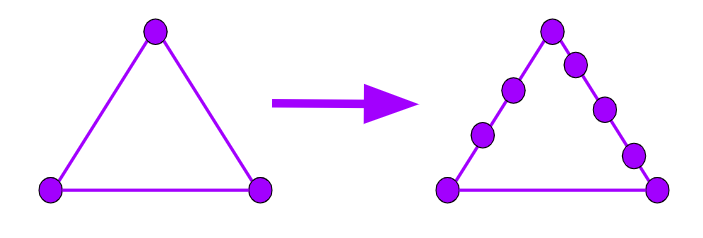
\includegraphics[scale=0.75]{Subdivision_Image.png}
   \end{myClosureOne}}
\end{center}}

{\begin{myIndent} \hTwo
   \uuline{Kuratowski's Theorem}: A graph is planar if and only if it does not contain a\\ subdivision of $K_5$ or $K_{3,3}$.
   \begin{myIndent} \hThree
      The proof for this is beyond the scope of this class.
      \newpage
   \end{myIndent}
\end{myIndent}}

Let $G$ be a plane graph. Then the faces of $G$ are the maximal connected regions of $\mathbb{R}^2 \setminus G$. We refer to the set of faces of $G$ as $F(G)$.

{\center \exOne
   \begin{myClosureOne}{4}
      The plane graph below has four faces: \retTwo 
      \exTwo\huge

      {\center\raisebox{-1em}{\tikz[scale=0.4,inner sep=5pt]{
         \tikzstyle{myCir}=[circle, fill, ultra thick, color=Purple];
         \tikzstyle{myLine}=[thick, line width=4pt, color=Purple];
   
         \node[myCir] (m) at (0:0) {};
         \node[myCir] (t) at (90:6) {};
         \node[myCir] (l) at (210:6) {};
         \node[myCir] (r) at (330:6) {};
   
         \draw (m) edge[myLine] (t);
         \draw (m) edge[myLine] (l);
         \draw (m) edge[myLine] (r);
         \draw (t) edge[myLine] (l);
         \draw (t) edge[myLine] (r);
         \draw (l) edge[myLine] (r);
   
         \node at (30:1.75) {$F_1$};
         \node at (150:1.75) {$F_2$};
         \node at (270:1.75) {$F_3$};
         \node at (45:5) {$F_4$};
      }}\par}
   \end{myClosureOne}
\par}
\retTwo

Beware that the same graph can have multiple plane drawings. \retTwo

If $G$ is connected, then the \udefine{boundary walk} of a face of $G$ is the shortest closed walk which uses every edge on the topological boundary of any face. \retTwo

The \udefine{degree} of a face is the length of its boundary walk.

{\center \exOne
   \begin{myClosureOne}{5.25}
      The middle face the graph below has degree $10$\dots \retTwo 
      \exTwo
      
      \begin{tabular}{p{2.5in} p{2in} p{0.2in}}
         {\center\raisebox{0em}{\tikz[scale=0.4,inner sep=5pt]{
            \tikzstyle{myCir}=[circle, fill, ultra thick, color=Purple];
            \tikzstyle{myLine}=[thick, line width=4pt, color=Purple];
            \useasboundingbox (-5,-5.75) rectangle (5, 5);

            \node[myCir] (t) at (90:6) {};
            \node[myCir] (tl) at (150:6) {};
            \node[myCir] (bl) at (210:6) {};
            \node[myCir] (b) at (270:6) {};
            \node[myCir] (br) at (330:6) {};
            \node[myCir] (tr) at (30:6) {};
            \node[myCir] (t2) at (90:2) {};
            \node[myCir] (b2) at (270:2) {};
   
            \draw (t) edge[myLine] (tl);
            \draw (tl) edge[myLine] (bl);
            \draw (bl) edge[myLine] (b);
            \draw (b) edge[myLine] (br);
            \draw (br) edge[myLine] (tr);
            \draw (tr) edge[myLine] (t);
            \draw (t) edge[myLine] (t2);
            \draw (b) edge[myLine] (b2);
            
         }}\par}
         &
         \retTwo
         The two vertices protruding inside the face have to be traversed twice by any walk going around the boundary of the internal face.
         &
      \end{tabular}
   \end{myClosureOne}
\par}
\retTwo

{\begin{myTindent}\begin{myTindent} \teachComment
   Proposition: The degree of the only face in a plane graph of a tree is twice the tree's number of edges.
\end{myTindent}\end{myTindent}}

\newpage

{\begin{myIndent} \hTwo
   \uuline{Handshaking Lemma}: ${\displaystyle\sum_{f \in F(G)}{\text{degrees}(f)} = 2|E(G)|}$

   {\begin{myIndent} \hThree
      Intution why:\\
      Each edge has a face on its left hand and right hand side (it might be the same face on both side). Thus the boundary walk of the face on the edge's left hand side will have to traverse that edge once, whereas the face on the edge's right hand side will also have to traverse that edge once. \retTwo
   \end{myIndent}}

   \uuline{Euler's formula}: Let $G$ be a connected plane graph. Then:
   
   {\center $|V(G)| - |E(G)| + |F(G)| = 2$\retTwo \par}

   {\begin{myIndent} \hThree
      Proof: (we shall prove by induction on the number of edges)\retTwo

      If $|E(G)| = |V(G)| - 1$, then $G$ is a tree and $|F(G)|=1$. So equality holds. \retTwo
      
      Now assume that the formula holds if $|E(G)| = |V(G)| + n - 1$ for some integer $n \geq 0$. Then consider a graph $G$ such that $|E(G)| = |V(G)| + n$.\\ We know that $G$ cannot be tree and so $G$ must contain a cycle $C$. If $e \in E(C)$,\\ then $G - \{e\}$ is still connected. So we can now apply our inductive\\ hypothesis to say that $|V(G - \{e\})| - |E(G - \{e\})| + |F(G - \{e\})| = 2$. \retTwo
      Note that $F(G - \{e\}) = F(G) - 1$ because by removing $e$, we removed the boundary seperating two different faces, thus merging them. Additionally, $V(G) = V(G - \{e\})$ and $E(G) = E(G - \{e\}) - 1$. So we can thus conclude that: $|V(G)| - (|E(G)| - 1) + (|F(G) - 1) = 2$. Or in other words:
      \[|V(G)| - |E(G)| + |F(G)| = 2\]
      \retTwo
   \end{myIndent}}

   \uuline{Theorem}: Let $G$ be a connected planar graph containing at least one cycle but\\ containing no cycles of length less than $g$. Then: \[|E(G)| \leq \dfrac{g}{g-2}\left(|V(G)| - 2\right)\]

   {\begin{myIndent} \hThree
      Proof: We know that the degree of each face $f \in F(G)$ is at least $g$. Thus, by the handshaking lemma, we get that $g|F(G)| \leq 2|E(G)|$. Now, inserting this into Euler's formula, we get that: \[|V(G)| - |E(G)| + \dfrac{2}{g}|E(G)| \geq |V(G)| - |E(G)| + |F(G)| = 2 \]
      This can then be manipulated to get the above formula. \retTwo
      
      \begin{myTindent} \hFour
         This upper bound is maximized when $g = 3$, thus giving a an upper bound not dependent on $g$ of:\[|E(G)| \leq 3|V(G)| - 6\]
         All in all, this is a neat necessary condition for a graph $G$ to be planar.\teachComment Beware though that this is not a sufficient condition. Some nonplanar graphs satisfy this inequality.
      \end{myTindent}
   \end{myIndent}}
\end{myIndent}}

\newpage

{\exOne
Some example calculations:
\begin{itemize}
   \item $K_5$: {\exTwo The minimum cycle in $K_5$ is of length $3$. So note: 
   
   {\centering ${\displaystyle \frac{3}{3-2}(|V(G)| - 2) = 9 < 20 = |E(K_5)|}$ \par}
   
   Thus, we have shown that $K_5$ can't be planar.} \retTwo

   \item Petersen Graph: {\exTwo The minimum cycle length in the Petersen graph is $5$. So note: 
   
   {\centering ${\displaystyle \frac{5}{5-2}(|V(G)| - 2) = 13\frac{1}{3} < 15 = |E(K_5)|}$ \par}
   
   Thus, we have shown that the Petersen graph can't be planar.}
   \retTwo
\end{itemize}
}

\markLecture{2/8/2024}

A \udefine{proper (vertex) coloring} of $G$ is a map $c: V(G) \longrightarrow S$ where $S$ is a set such that\\ $c(u) \neq c(v)$ if $\{u, v\} \in E(G)$. \retTwo

The \udefine{cromatic number} $\chi(G)$ is the minimum $k$ for which $G$ has a proper $k$-coloring. \retTwo

{\begin{myIndent} \hTwo

   A graph $G$ is \udefine{$d$-degenerate} if every induced subgraph of $G$ has a vertex of degree at most $d$. \retTwo
   \uuline{Lemma}: If $G$ is $d$-degenerate, then $\chi(G) \leq d + 1$.
   
   {\begin{myIndent} \hThree
      Proof:\\
      Firstly, observe that if a graph $G$ is $d$-degenerate, then any subgraph resulting by removing vertices from $G$ will also be $d$-degenerate. \retTwo
      Also, observe that for any induced subgraph $H$ of $G$, we clearly have that $\delta(H) \leq d$. Therefore, assuming $H$ is nonempty, we know there exists a vertex $v \in V(H)$ such that $d(v) \leq d$. \retTwo
      Using the above two observation, we can do induction over a $d$-degenerate graph as follows:
      {\begin{myIndent} \hFour
         For each integer $i \in \{1,\ldots,|V(G)|\}$, remove a vertex $v_i$ from\\ $H_i = G - \{v_1, \ldots, v_{i-1}\}$ satisfying the property that $d_{H_i}(v_i) \leq d$. \retTwo

         Doing this, we will eventually be left with an empty graph. This graph\\ obviously has a proper coloring using at most $d + 1$ colors.\retTwo Next, consider adding vertices back in. For any $i \in \{1,\ldots,|V(G)|\}$, we shall inductively assume that $G - \{v_1, \ldots, v_{i-1}, v_i\}$ has a proper coloring using less than $d + 1$ colors. Then, because we specified that $v_i$ has at most a degree of $d$ in $G - \{v_1, \ldots, v_{i-1}\}$, we know there is at least one available color to assign $v_i$. So $G - \{v_1, \ldots, v_{i-1}\}$ has a proper coloring using at most $d + 1$ colors. $\blacksquare$
      \end{myIndent}}
   \end{myIndent}}

   \newpage

   \uuline{Brook's Theorem}: If $G$ is a connected graph, then $\chi(G) \leq \Delta G$ unless $G$ is an odd cycle or a complete graph.

   {\begin{myIndent} \hThree
      Proof: (we shall proceed by induction on the number of vertices in $G$)\retTwo

      To start, consider that $\chi(K_n) = \Delta(K_n) + 1$. Similarly for an odd cycle $C$, we have that $\chi(C) = \Delta(C) + 1$. Hence, this is why Brook's theorem specifies that $G$ is not one of the above graphs. Additionally, note that if $\Delta G < 3$, then the theorem is obviously true. So, we only need to focus on when $\Delta G \geq 3$. \retTwo

      Now, note that we may assume for all $v \in V(G)$ that $G - \{v\}$ is connected. 
      {\begin{myIndent} \hFour
         After all, if $G - \{v\}$ was not connected, then we could write $G$ as the\\ union of two smaller connected graphs: $G_1$ and $G_2$ such that\\ $V(G_1) \cap V(G_2) = \{v\}$. Now if $G_i$ is an odd cycle or a complete graph,\\ then we know $\chi(G_i) = \Delta(G_i) + 1$. However, then $\Delta(G_i) \leq \Delta(G) - 1$ because the degree of the vertex connecting $G_i$ to the rest of $G$ is equal to $\Delta(G_i)$. Meanwhile if $G_i$ is not an odd cycle or complete graph,\\ then we can inductively prove Brook's Theorem for $G_i$ to get that\\ $\chi(G_i) \leq \Delta(G_i) \leq \Delta(G)$. In either case, we will get a coloring over $G_i$ using at most $\Delta G$ colors. \retTwo

         So $G_1$ and $G_2$ both have colorings with at most $\Delta(G)$ colors. By setting $v$ in both graphs to have the same color, we  can then merge the colorings of $G_1$ and $G_2$ to get a suitable coloring of $G$.
         \retTwo
      \end{myIndent}}

      Thus, assume that $G - \{v\}$ is connected for all $v \in V(G)$. Then, if\\ $G \neq K_{\Delta(G) + 1}$, we can pick vertices $v_1$, $v_{n-1}$ and $v_{n}$ such that\\ $\{v_1, v_{n-1}\} \in E(G)$, $\{v_1, v_{n}\} \in E(G)$, and $\{v_{n-1}, v_{n}\} \notin E(G)$. \retTwo

      \uuline{Case 1}: Suppose $H = G - \{v_n\} - \{v_{n-1}\}$ is connected. Then, we can order the vertices of $H$: $v_1, v_2, \ldots, v_{n-2}$ so that for $i \geq 2$, $v_i$ always has at least one neighbor $v_j$ where $j < i$.
      {\begin{myTindent}\begin{myTindent} \teachComment
         This was proven in a homework exercise\dots\retTwo
      \end{myTindent}\end{myTindent}}

      Assign $v_n$ and $v_{n-1}$ the color $1$. Then, considering our graph $G$, since $v_i$ has at most $\Delta(G) - 1$ neighbors $v_j$ where $i < j$, we can iterate from $v_{n-2}$ to $v_2$, assigning whatever color is available to each vertex. After all, it is guarenteed that we will not have assigned all $\Delta(G)$ colors to the neighborhood of $v_i$ yet since we could have only assigned $\Delta(G) - 1$ colors at most.
      {\begin{myTindent} \hFour
         If $v_i$ is neighbors with $v_n$ or $v_{n+1}$ then that just means it isn't neighbors with one or two more $v_j$ in our ordering. So, this doesn't affect our conclusion. \retTwo
      \end{myTindent}}

      Also, the number of colors assigned in $N(v_1)$ is at most $\Delta(G) - 1$ since two of $v_1$'s neighbors are assigned the same color. So we can assign it a remaining color afterwards. Hence $G$ has a proper coloring. \retTwo

      \newpage

      \uuline{Case 2}: Now suppose $H = G - \{v_n\} - \{v_{n+1}\}$ is disconnected. Then we may view $G$ as the union of two smaller connected graphs $G_1$ and $G_2$ such that $V(G_1) \cap V(G_2) = \{v_n, v_{n+1}\}$. By the same type of induction that we did earlier, we can prove that $G_1$ and $G_2$ can be covered by at most $\Delta(G)$ colors. So, choose a coloring such that $v_n$ and $v_{n+1}$ are assigned the same colors in both $G_1$ and $G_2$. Then, we can merge the two colorings to get a proper coloring of $G$. $\blacksquare$
   \end{myIndent}}
   \retTwo
   Note that $\Delta(G)$ can differ greatly from $\chi(G)$. For instance, bipartite graphs are always $2$-colorable no matter how many edges they have.
\end{myIndent}}

\mySepTwo

A \udefine{maximal planar graph} is a graph that is planar but the addition of any edge\\ results in a non-planar graph. Similarly, a \udefine{maximal plane graph} is a plane drawing of a maximal planar graph. \retTwo

{\begin{myIndent} \hTwo
   \uuline{Theorem}: Every planar graph has a vertex $v$ of degree at most $5$.
   {\hThree 
   \begin{myIndent}
      Proof:\\
      If $G$ is planar, then $|E(G)| \leq 3|V(G)| - 6$. However,\\ ${\displaystyle \sum_{v\in V(G)}{d_G(v)} = 2|E(G)| \leq 6|V(G)| - 12 < 6|V(G)|}$.\retTwo So not every vertex in $G$ can have a degree of $6$ or more. \retTwo
   \end{myIndent}}
\end{myIndent}}

A \udefine{contraction} of an edge $\{a, b\}$ in a graph $G$, notated as $G \slash \{a, b\}$, is the graph\\ obtained by adding a vertex $x$ to $G - \{a\} - \{b\}$ so that $x$ is adjacent to all vertices in $N_G(a) \cup N_G(b)$. An important property of contractions is that if $G$ is planar, then $G \slash \{a, b\}$ is also planar.\retTwo

{\center\exOne
\begin{myClosureOne}{5.8}
   What a contraction looks like:
   
   {\centering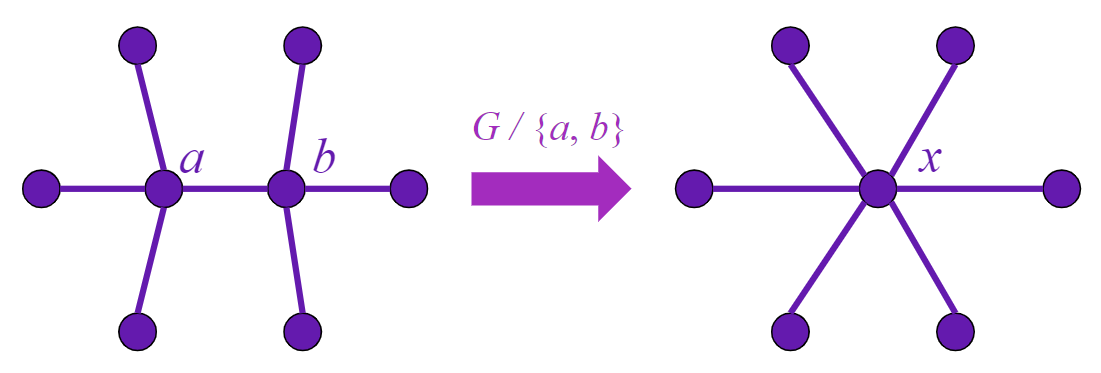
\includegraphics[scale=0.75]{Contraction_Image.png}\par}
\end{myClosureOne}
\par}

\newpage

{\begin{myIndent} \hTwo
   \uuline{The $5$-color Theorem}:  If $G$ is a planar graph, then $\chi(G) \leq 5$.
   {\hThree 
   \begin{myIndent}
      Proof:\\
      If $|V(G)| \leq 5$, then we may simply assign all vertices different colors to show that $\chi(G) \leq 5$. So, consider when $|V(G)| \geq 6$.\retTwo

      Then if $\delta(G) \leq 4$, we know there exists $v \in V(G)$ such that $d_G(v) \leq 4$. So, by induction we can find a proper $5$-coloring of $G - \{v\}$. And because $v$ has at most $4$ neighbors, there is at least one color left over to assign $v$ afterwards.\\ Meanwhile, because of the previous theorem, we know that any induced\\ subgraph of $G$ will have a minimum degree of at most $5$. So, the only \\non-trivial case we need to prove is when $\delta(G) = 5$. \retTwo

      Thus, assume there exists a vertex $v \in V(G)$ such that $d(v) = 5$. Since $K_5$ is not planar, there exists some pair of vertices: $a, b \in N_G(v)$ which are not\\ adjacent. Define $H = G \slash \{a, b\}$ with a new vertex $w$ adjacent to\\ $N_G(v) \cup N_g(a)$. \retTwo

      Next contract $H$ again, defining $I = H \slash \{b, w\}$ with a new vertex $x$ adjacent to $N_H(w) \cup N_H(b)$. Note that $I$ and $H$ are planar. Thus, since $I$ is a planar graph with less vertices than $G$, we can do induction to find a proper $5$-coloring of $I$. We'll call this coloring $c$. \retTwo

      For each $y \in V(I) \cap V(G)$, define $c^\prime(y) = c(y)$. This effectively gives a proper coloring of $G - {a} - {b} - {v}$. Then assign $c^\prime(a) = c^\prime(b) = c(x)$. We can do this because we chose $a$ and $b$ to not be adjacent and because none of $a$ and $b$'s neighbors could have been assigned $c(x)$. And finally, because $a$ and $b$ in $N(v)$ have been assigned same color, there is at least one color which we can assign to $v$. $\blacksquare$ \retTwo
   \end{myIndent}}
\end{myIndent}}

\mySepTwo

\markLecture{2/13/2024}

\uuline{\textbf{The Art Gallery Problem}}:\\
Let $R$ be a region in the plane bounded by a polygon. Also, define that two points are "\textit{mutually visible}" if there exists a straight line between them that is contained entirely in $R$. Then, what is the smallest size of a set of points $S$ in $R$ such that every point in $R$ is mutually visible to a point in $S$. 

\newpage

\exOne
\begin{myClosureOne}{6.2}
   In terms of the art gallery analogy, $R$ is the floor plan of an art gallery and $|S|$ is the number of guards you've hired to guard the gallery.
   Here are some example galleries with guards:\exTwo\color{BrickRed}
   
   {\centering
   \begin{tabular}{p{1.4in} p{1.4in} p{1.4in} p{1.4in}}
      {\centering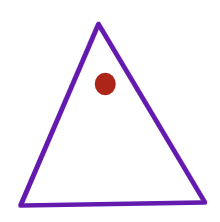
\includegraphics[scale=0.6]{art_gallery_1.png} \newline
      $3$ edges,
      $1$ guard \par} &
      {\centering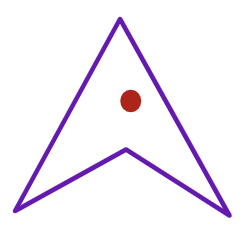
\includegraphics[scale=0.6]{art_gallery_2.png} \newline
      $4$ edges,
      $1$ guard \par} &
      {\centering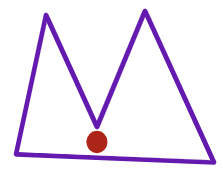
\includegraphics[scale=0.6]{art_gallery_3.png} \newline
      $5$ edges,
      $1$ guard \par} &
      {\centering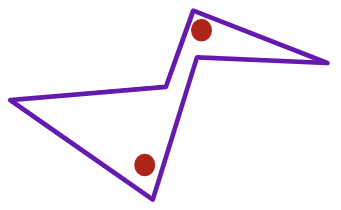
\includegraphics[scale=0.6]{art_gallery_4.png} \newline
      $6$ edges,
      $2$ guard \par} \\
   \end{tabular}\par}
\end{myClosureOne}

\retTwo
\hOne

{\begin{myIndent} \hTwo
   \uuline{Art Gallery Theorem}: For an $n$-sided polygon, one needs to include at most $\lfloor \frac{n}{3} \rfloor$ many points in $S$ in order to have that every point in $R$ be mutually visible with a point in $S$.

   \hThree
   \begin{myIndent}
      Proof:\\
      Consider triangulating $R$. In other words, add straight edges between vertices of $R$ in order to partition $R$ into a bunch of triangular regions. \retTwo
      Having done that, now consider the graph $G$ whose vertices are the vertices of $R$ and whose edges are the boundaries of the triangles of our triangulation of $R$. We can prove that $\chi(G) = 3$. \retTwo

      {\hFour
      \begin{myIndent}
         When $n = 3$, we have that $G$ consists of a single triangle. So $\chi(G) = 3$. \retTwo
         Now we proceed by induction. Assume that for $n > 3$, we know that \\$\chi(G) = 3$ if $R$ has less than $n$ sides. Therefore, we now consider a graph $G$ made from an $n$-sided polygon. Let $\{u, v\}$ be any edge of $G$ not on the boundary of the infinite face. Importantly, we know such a side will exist\\ because $n > 3$. Then, we can partition $G$ into two subgraphs $G_1$ and $G_2$ such that $V(G_1) \cap V(G_2) = \{u, v\}$ and $E(G_1) \cup E(G_2) = E(G)$. \retTwo

         $G_1$ and $G_2$ are the triangulations of some polygon with less than $n$ sides.\\ Therefore by strong induction, there exists the proper vertex $3$-colorings:\\ $c_1: V(G_1) \rightarrow \{1, 2, 3\}$, and $c_2: V(G_2) \rightarrow \{1, 2, 3\}$. Shifting around the colors so that $c_1(u) = c_2(u)$ and $c_1(v) = c_2(v)$, we can then define a proper $3$-coloring of all $G$. So $\chi(G) \leq 3$. \retTwo

         Since $G$ obviously can't be colored by 2 or less colors since the triangles in $G$ need three colors, we thus conclude that $\chi(G) = 3$. \retTwo
      \end{myIndent}}

      Having shown that $G$ has a $3$-coloring, now note that in that $3$-coloring, the three vertices enclosing any triangular face of $G$ must all have a different color assigned to them. Additionally, every point in a triangle is mutually visible to another point in that triangle.
      \newpage
      Letting the least assigned color be called $i$, make $S$ the set of locations of vertices which were assigned the color $i$. Then any point in any of the triangles partioning $R$ is mutually visible to a point in $S$. Also, $|S|$ is at most $\lfloor \frac{n}{3} \rfloor$. $\blacksquare$ \retTwo
   \end{myIndent}
\end{myIndent}}

Some other problems related to the art gallery problem are:
\begin{myIndent}
   \begin{itemize}
      \item The rectilinear art gallery problem.
      {\begin{myIndent} \hTwo
         In this version of the problem, all angles between sides must be right angles. As it turns out, with this restriction on $R$ we only need $\lfloor \frac{n}{4} \rfloor$\\ points in $S$ so that every point in $R$ is mutually visible with a point in $S$. However, we aren't proving that in this class.
      \end{myIndent}}

      \item The 3d art gallery problem
      \item The non-polygon art gallery problem
   \end{itemize}
\end{myIndent}

\mySepTwo


{\begin{myIndent} \hTwo
   \uuline{The 4-color Theorem}: If $G$ is a planar graph, then $\chi(G) \leq 4$.
   
   \begin{myIndent} \hThree
      Unfortunately, no short proof of this is known. The quickest proof  considers 633 different cases. \retTwo
   \end{myIndent}
\end{myIndent}}

Let $G$ be a plane graph. To get the \udefine{dual} of $G$, denoted $G^*$, represent each face $f \in F(G)$ as a vertex in $G^*$ and draw it inside its corresponding face in $G$. Then, for each edge $e \in E(G)$, draw an edge $\{f_1, f_2\} \in E(G^*)$ such that $e$ is between the faces $f_1$ and $f_2$ of $G$ and $\{f_1, f_2\}$ is drawn to only intercept $e$ at one point. \retTwo \retTwo

{\centering \exOne
   \begin{myClosureOne}{5.25}
      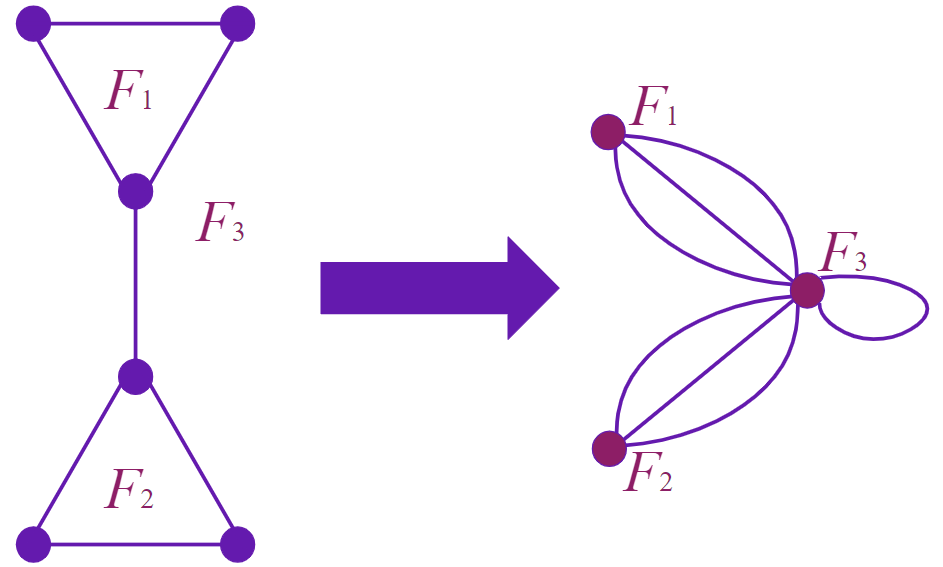
\includegraphics[scale=0.6]{Dual_Image.png}
      \\ Note that {\color{RedViolet} $G^*$} is a planar multigraph.\\
   \end{myClosureOne}
\par}

\newpage

{\begin{myIndent} \hTwo
   \uuline{Proposition}: If $G$ is connected, then $(G^*)^* \cong G$. In other words, while $(G^*)^*$ might be drawn in the plane differently from $G$, both graphs will have the same vertex, edge, and face sets.
   
   {\begin{myIndent} \hThree
      The proof for this is beyond the scope of this class (and requires math I don't know yet). \retTwo
   \end{myIndent}}
\end{myIndent}}

The significance of the above proposition is that by taking the dual of a connected plane graph $G$, we can convert the faces of $G$ into vertices and the vertices of $G$ into faces.
{\begin{myDindent}\begin{myDindent} \exOne
   Application: giving a proper coloring of the faces of $G$ is equivalent to giving a proper coloring of the vertices of $G^*$.
\end{myDindent}\end{myDindent}}

\mySepTwo

Here is one notable approach to the four color theorem: \retTwo

A graph $G$ is \udefine{$k$-edge-connected} if for every set $X$ of less than $k$ edges, $G - X$ is still connected.

{\begin{myIndent} \hTwo
   \uuline{Proposition}: $G^*$ is simple if and only if $G$ is $3$-edge-connected.

   {\begin{myIndent} \hThree
      Proof: (by contrapositive)\\
      ($\Longrightarrow$) If $G$ is $1$-edge-connected, then we know there is a bridge $\{u, v\}$ in $G$. That bridge must have the same face on either side of it or else there'd be an alternate path going from $u$ to $v$, thus contradicting that $\{u, v\}$ is a bridge. This then means that $G^*$ must have a loop. So $G^*$ is not simple.\retTwo

      Now consider if $G$ is $2$-edge-connected. In that case there exists edges $e_1$ and $e_2$ which when both removed split $G$ into two components. Let $e_1$ be on the boundary of $f_1$ and $f_2$. The effect of subtracting $e_1$ from $G$ is that we merged only those two faces in the graph $G - e_1$. Meanwhile, we know that $e_2$ must be a bridge in $G - e_1$. Therefore it must have the same face on either side of it. However, $e_2$ wasn't a bridge in $G$. This tells us that $e_2$ must also be on the boundary of $f_1$ and $f_2$. So $f_1$ and $f_2$ must share two edges on their boundaries, which in turn means  that $G^*$ is not simple.\retTwo

      ($\Longleftarrow$) If $G^*$ has a loop, then that means there is an edge in $G$ not on the boundary of two distinct faces. Then that edge is a bridge, which means that $G$ is $1$-edge-connected.\retTwo

      If $G^*$ has multiple edges going between two vertices, then two faces of $G$ share more than one edge. By removing one of those shared edges, all the remaining shared edges become bridges. Hence, removing two shared edges disconnects the graph. So $G$ is $2$-edge connected.
   \end{myIndent}}
\end{myIndent}}

\newpage

Now the $4$-color theorem is obviously true if $|V(G)| < 4$. Thus, to prove the $4$-color theorem, we can focus exclusively on graphs with at least $4$ vertices. Additionally, it is enough to prove the $4$-color theorem for maximal planar graphs (i.e. a planar graph with as many edges as possible). After all, removing edges does not make a coloring invalid.\retTwo

{\begin{myIndent}\hTwo
   Observation 1: $G$ is a maximal planar graph if and only if every face of $G$ is a triangle. \retTwo

   Observation 2: The dual of any maximal planar graph with at least $4$ vertices is a simple planar $3$-edge-connected cubic graph.
   {\begin{myIndent} \hThree
      Let $G$ be a maximal planar graph. Then as every face of $G$ is a triangle, every face of $G$ has three neighbors. Hence $G^*$ is cubic.\retTwo

      Additionally, as every face of $G$ must be a triangle, if two faces share two edges $\{u, v\}$ and $\{v, w\}$, then they must also both have an edge $\{u, w\}$. Since the graph $G$ has at least four vertices, we know that $G$ is not just a single triangle. Hence, the only way for both faces to have an edge $\{u, w\}$ would be if $G$ was a multigraph (something we haven't allowed for). So we conclude that $G^*$ has at most one edge going between any two vertices. \retTwo

      Since $G$ and thus $(G^*)^*$ is assumed to be simple since we did not indicate otherwise, we know that $G$ is $3$-edge-connected.\retTwo
   \end{myIndent}}

   Observation 3: The dual of any planar $3$-connected cubic graph is a maximal planar graph.

   {\begin{myIndent} \hThree
      Let $G$ be a planar $3$-connected cubic graph. Then $G^*$ being $3$-connected\\ means that $G^*$ is simple (so it makes sense to even ask if $G^*$ is a maximal planar graph). Additionally, $G$ being cubic means that every face of $G^*$ is a\\ triangle. So $G^*$ is a maximal planar graph.
      \retTwo
   \end{myIndent}}
\end{myIndent}}

This then leads to the following theorem:

{\begin{myIndent} \hTwo
   \uuline{Theorem}: Every planar graph $G$ is $4$-colorable if and only if every $3$-connected cubic planar graph is $3$-edge colorable.

   {\begin{myIndent} \hThree
      Proof:\\
      ($\Longrightarrow$) Let $G$ be a $3$-connected cubic planar graph. Then we know that $G^*$ is a maximal planar graph. If $G^*$ is $4$-colorable, then we can properly color the vertices of $G^*$, which is equivalent to properly coloring the faces of $G$. \retTwo

      Let $c: F(G) \rightarrow \{1, 2, 3, 4\}$ be a proper face coloring of $G$. Then because $G$ is $3$-connected, we know that no edge in $G$ is a bridge. So, every edge in $G$ is between two faces which are colored differently.
      
      \newpage
      We now define the following $3$-edge-coloring of $G$:\\
      \begin{myIndent}
         If $e$ is between face colors $1$ and $2$, or $3$ and $4$, define $c^\prime(e) = 1$.\\
         If $e$ is between face colors $1$ and $3$, or $2$ and $4$, define $c^\prime(e) = 2$.\\
         If $e$ is between face colors $1$ and $4$, or $2$ and $3$, define $c^\prime(e) = 3$.\\
      \end{myIndent}

      Hence $\chi^\prime(G) = 3$. \retTwo \retTwo
      
      ($\Longleftarrow$) Now let $G$ be a maximal plane graph. If $G^*$ is $3$-edge-colorable, then there exists an edge coloring $c^\prime: E(G^*) \rightarrow \{1, 2, 3\}$. \retTwo

      Consider the set $H_1 = \{e \in E(G^*) \mid c^\prime(e) \in \{1, 2\}\}$. $H_1$ must\\ consist of some number of disjoint cyles which span $G^*$. Similarly,\\ $H_2 = \{e \in E(G^*) \mid c^\prime(e) \in \{1, 3\}\}$ must also consist of some number of\\ disjoint cycles which span $G^*$. Note that $H_1 \cup H_2$ span $G^*$. So every edge is on the boundary of a cyle of either $H_1$ or $H_2$.\retTwo

      Define $c_1(f)$ such that $c_1(f) = 1$ if $f$ is in the interior of a cycle of $H_1$, whereas $c_1(f) = 2$ if $f$ is not in the interior of a cycle of $H_1$. Similarly define $c_2(f)$ but using $H_2$. \retTwo

      Now we define the following face coloring of $G^*$:
      \begin{myIndent}
         $c(f) = 1$ if $(c_1(f), c_2(f)) = (1, 1)$\\
         $c(f) = 2$ if $(c_1(f), c_2(f)) = (1, 2)$\\
         $c(f) = 3$ if $(c_1(f), c_2(f)) = (2, 1)$\\
         $c(f) = 4$ if $(c_1(f), c_2(f)) = (2, 2)$\\
      \end{myIndent}

      Then $c$ is a proper $4$-face-coloring of $G^*$. So, we in turn know that $G$ has a proper $4$-vertex-coloring.

      \retTwo
   \end{myIndent}}
\end{myIndent}}


{\centering{\myComment
\begin{tabular}{ p{5.8in} }
   \hline \\
   Here's a quick useful calculation for the homework that the professor gave us:
   {\begin{myIndent} \teachComment
      Let $G$ be a maximal planar graph with $n$ vertices. By the handshaking lemma, we know that $3|F(G)| = 2|E(G)|$. And since $G$ is obviously connected, we can thus say that: $|V(G)| - |E(G)| + |F(G)| = n - \frac{1}{2}|F(G)| = 2$. So, $|F(G)| = 2n - 4$. Plugging this into Euler's formula again, we then get that $|E(G)| = 3n - 6$. \retTwo

      As a result, we know that $G^*$ has $2n - 4$ vertices and $3n - 6$ edges.
   \end{myIndent}}
   \\ \hline \\
\end{tabular}}\par}

\newpage

\markLecture{2/15/2024}

Let $\mathcal{F}$ be any family of graphs.\\
The \udefine{external numbers / Turán numbers} for $\mathcal{F}$ are the quantities $\exNums{n, \mathcal{F}}$ which\\ denote the maximum number of edges in an $n$ vertex graph not containing any graph in $\mathcal{F}$.\retTwo

We call a graph that does not contain any member of $\mathcal{F}$ an \udefine{$\gfam{F}$-free graph}.

A \udefine{$k$-core} of a graph $G$ is the graph obtained through the following algorithm:
{\begin{myIndent} \hTwo
   1. Let $X$ be the set of vertices removed from $G$ in previous steps. \retTwo 
   2. If there is no vertex $v \in V(G - X)$ with degree less than $k$ in $G - X$, then you are done as $G - X$ is a $k$-core of $G$. \retTwo
   3. Otherwise, add $v$ to the set $X$ and go back to step 2. \retTwo
\end{myIndent}}

If not empty, a $k$-core is the largest subgraph of $G$ with minimum degree at least $k$.
{\begin{myTindent} \teachComment
   The order in which vertices are removed does not matter. The $k$-core of a graph is unique. \retTwo
\end{myTindent}}

{\begin{myIndent} \hTwo
   \uuline{Lemma}: If $G$ is an $n$-vertex graph with more than $(k - 1)n -
   \binom{k}{2}$ edges, then $G$ has a nonempty $k$-core.

   {\begin{myIndent} \hThree
      Proof:\\
      If $\delta(G) \geq k$, we're done. So, assume that there is a vertex $v_1 \in V(G)$ with $d(v_1) \leq k - 1$. Then:
      
      {\center$|E(G - \{v\})| > (k-1)n - \binom{k}{2} \cyPen{- (k - 1)} = (k-1)(n \cyPen{- 1}) - \binom{k}{2}$\retTwo\par}

      Now if $n = k$, then $|E(G)| > (k-1)k - \binom{k}{2} = \binom{k}{2}$. But that would mean that $G$ has more edges than $K_n$, which is impossible. So, we know that $n > k$. Therefore, it makes sense to consider repeating the above step $n - k$ times. Having done that, we will once again get that there are more than $(k - 1)(k) - \binom{k}{2}$ edges remaining. However, that is impossible as a $k$ vertex graph can't have more than $\binom{k}{2}$ edges. Hence, we conclude that the algorithm must have terminated before all $n - k$ steps could be done. \retTwo
   \end{myIndent}}

   \uuline{Corollary}: If $G$ is a graph with $n$ vertices and more than $(k - 1)n - \binom{k}{2}$ edges, then $G$ contains a cycle of length at least $k + 1$ unless $G = K_k$.

   {\begin{myIndent} \hThree
      Proof:\\
      Let $H \subseteq G$ be a non-empty $k$-core in $G$. Since $\delta(H) \geq k$, $H$ contains a cycle of length at least $k + 1$. Thus so does $G$. $\blacksquare$
      \retTwo
   \end{myIndent}}
\end{myIndent}}

\newpage

A \udefine{cut}: $(A, B)$, of a graph $G$ is a spanning subgraph of $G$ such that such that $V(G)$ is partitioned into two sets $A$ and $B$ and an edge $\{a, b\} \in E(G)$ is only included in the cut if $a \in A$ and $b \in B$. \retTwo

A \udefine{max cut} is a cut with as many edges as possible.


{\begin{myIndent} \hTwo
   \uuline{Theorem}: Every graph with $m$ edges has a cut with at least $\sfrac{m}{2}$ edges.

   {\begin{myIndent} \hThree
      Proof:\\
      Let $G$ have $m$ edges. On each vertex of $G$, flip a fair coin. 
      Then, let $A$ be the set of vertices which have heads and let $B$ be the set of vertices which have tails. That way, $(A, B)$ is a cut.
      \retTwo

      Since the assignment of each vertex is independent from the assignment of any other vertex, we have that there is a $\frac{1}{2}$ probability of any edge being included in the cut. Thus, the mean number of edges between $A$ and $B$ is: 
      \[\sum\limits_{e \in E(G)}{\mathbb{P}(e\text{ is in the cut})} = \sum\limits_{i=1}^m\frac{1}{2} = \frac{1}{2}m\]

      This implies that some cut $(A, B)$ of $G$ must have at least $\sfrac{m}{2}$ edges. (It also implies some cut has at most $\sfrac{m}{2}$ edges.) \retTwo
   \end{myIndent}}
\end{myIndent}}

\mySepTwo

{\begin{myIndent} \hTwo
   \uuline{Erd\H{o}s-Gallai Theorem}: Let $k \geq 1$, \hspace{0.2em} $n \geq 1$, and let $G$ be an $n$-vertex $P_k$-free graph. Then $|E(G)| \leq (k-1)\frac{n}{2}$ with equality if and only if $k$ divides $n$ and every component of $G$ is $K_k$.

   {\begin{myIndent} \hThree
      Proof: (we proceed by induction)\retTwo

      Base Case:
      {\begin{myIndent} \hFour
         If $k = 1$, then $\exNums{n, P_k} = 0 = (k-1)\frac{n}{2}$. Thus, the theorem is trivially true. \retTwo

         If $n \leq k$, then $\exNums{n, P_k} = E(K_n) = (n-1)\frac{n}{2} \leq (k - 1)\frac{n}{2}$. Specifically, equality holds if $n = k$. \retTwo
      \end{myIndent}}

      Inductive step: (assume the theorem holds if $|V(G)| < n$)
      {\begin{myIndent} \hFour
         Suppose $G$ is an $n$ vertex $P_k$-free graph. \retTwo

         If $G$ is disconnected, then there are two disjoint subgraphs $G_1$ and $G_2$ such that $G = G_1 + G_2$. Furthermore, $G$ is $P_k$-free if and only if $G_1$ and $G_2$ are both $P_k$-free. Let $|V(G_1)| = n_1$ and $|V(G_2)| = n_2$. Because $n_1, n_2 < n$, we know by induction that for $G_1$ and $G_2$ to be $P_k$-free, we must have that $E(G_1) \leq (k - 1)\frac{n_1}{2}$ and that $E(G_2) \leq (k - 1)\frac{n_2}{2}$. Therefore:
         
         {\center $E(G) \leq (k - 1)\frac{n_1}{2} + (k - 1)\frac{n_2}{2} = (k - 1)\frac{n}{2}$ \par}
         
         \newpage

         Now we suppose $G$ is connected.\retTwo

         If $G$ has a vertex $v$ of degree less than $\frac{k}{2}$, then consider that because $G - \{v\}$ must be $P_k$ free, we know by induction that $|E(G - \{v\})| \leq (k-1)\frac{n-1}{2}$. This in turn means that:
         {\center $|E(G)| \leq (k-1)\frac{n-1}{2} + \frac{k-1}{2} = (k-1)\frac{n}{2}$. \retTwo\par}

         Also, note that by induction, $|E(G - \{v\})| = (k-1)\frac{n-1}{2}$ if and only if $|E(G - \{v\})|$ is a bunch of disjoint $K_k$ components. But in that case, if\\ $d(v) \geq 1$, then $G$ cannot be $P_k$-free. So, we can actually conclude that\\ $|E(G)| < (k-1)\frac{n}{2}$.

         {\center{\rule{4in}{0.25mm}}\\ [8pt]\par}

         Meanwhile, if $\delta(G) \geq \frac{k}{2}$, then assume towards a contradiction that\\ $|E(G)| > (k - 2)\frac{n}{2}$. That way, by induction on $k$, we can conclude that $G$ has a path $P$ of length $k - 1$
         {\begin{myTindent} \myComment
            This was why we included the base case of when $k = 1$. \retTwo
         \end{myTindent}}

         If $P$ can be extended, then we have a contradiction as $G$ is not $P_k$ pathless. So assume $G$ can't be extended. Then, using the same trick as we used\\ previously to prove Dirac's Theorem (pages 14 and 15), we can turn $P$ into a cycle of length $k - 1$. But this gives another contradiction because $G$ is\\ connected. So, there must be a vertex adjacent to our cycle of length $k$, which means that we can remove an edge of the cycle and add an edge to that adjacent vertex to get a path of length $k$ in $G$.
         \retTwo

         So, when $\delta(G) \geq \frac{k}{2}$, we have shown that $|E(G)| \leq (k - 2)\frac{n}{2} < (k - 1)\frac{n}{2}$.

         {\center{\rule{4in}{0.25mm}}\\ [8pt]\par}

         Notably, $|E(G)| = (k-1)\frac{n}{2}$ if and only if the only induction we ever did was considering if $G$ was disconnected, and if the only base case we ever reached was for when a subgraph equals $K_k$. So equality holds if and only if $k$ divides $n$ and every component of $G$ is $K_k$.
      \end{myIndent}}
   \end{myIndent}} 
\end{myIndent}}

\mySepTwo

\markLecture{2/20/2024}

The \udefine{Turán graph} $T_r(n)$ has $n$ vertices which are partitioned into $r$ sets of size $\lfloor \frac{n}{r} \rfloor$ or $\lceil \frac{n}{r} \rceil$ such that $E(T_r(n))$ consists of every possible edge going between different partitions.

{\begin{myIndent} \hTwo
   Observe: $K_{r+1} \nsubseteq T_r(n)$ because $\chi(K_{r+1}) = r + 1 > r = \chi(T_r(n))$ for any $n$. \retTwo

   If $r \mid n$, then by handshaking lemma:
   
   {\center$e(T_r(n)) = \left(\frac{n}{r}(r - 1)\right)\frac{n}{2} = \binom{r}{2}\frac{n^2}{r^2} = \frac{n^2}{2}(1 - \frac{1}{r})$\par}
   
   \newpage
   
   \uuline{Turán's Theorem}: For all $n \geq 1$ and $r \geq 2$, $\exNums{n, K_{r+1}} = e(T_r(n))$. Also, if $G$ is a $K_{r+1}$-free graph on $n$ vertices and $e(G) = e(T_r(n))$, then $G = T_r(n)$.
   {\begin{myIndent} \myComment
      \begin{myTindent}\begin{myDindent}
         In other words, $T_r(n)$ is the unique maximal graph. \retTwo
      \end{myDindent}\end{myTindent}

      \hThree Proof: (we proceed by induction)\retTwo

      Base Case:
      {\begin{myIndent} \hFour
         When $n \leq r$, we clearly have that $\exNums{n, K_{r+1}} = e(K_n)$. However, we also have $T_r(n) = K_n$ when $n \leq r$. Thus, Turán's theorem is clearly true when $n \leq r$.
         \retTwo
      \end{myIndent}}

      Inductive Step: (assume the theorem holds when $r \leq |V(G)| < n$)
      {\begin{myIndent} \hFour
         Assume $G$ is a $K_{r+1}$-free graph such that $e(G) \geq e(T_r(n))$. \retTwo
         Remove edges from $G$ until we get a graph $G^\prime$ with $e(G^\prime) = e(T_r(n))$. Then let $v$ be a vertex of $G^\prime$ of minimum degree. We know that $d_{G^\prime}(v) \leq \delta(T_r(b))$ because if this weren't the case, then $G^\prime$ would have to have more edges than $T_r(n)$ by the handshaking lemma. Therefore:
         
         {\center$e(G^\prime - \{v\}) \geq e(T_r(n)) - \delta(T_r(n)) = e(T_r(n-1))$. \retTwo\par}

         But now by induction, we know that $G^\prime - \{v\}$ is $K_{r+1}$-free only if\\ $e(G^\prime - \{v\}) \leq e(T_r(n-1))$. Therefore $e(G^\prime - \{v\}) = e(T_r(n-1))$. Furthermore, this tells us by induction that $G^\prime - \{v\} = T_r(n-1)$.
         \retTwo

         Next, we try to fit $v$ back into $G^\prime - \{v\} = T_r(n-1)$. Let $W_1, \ldots, W_r$ be the partitions of $G^\prime - \{v\}$. If $N_{G^\prime}(v) \cap W_i \neq \emptyset$ for all $i \in \{1, \ldots, r\}$, then by picking one $v_i$ from each $W_i \cap N_{G^\prime}(v)$, we get that $\{v, v_1, \ldots, v_r\}$ induces a $K_{r+1}$ subgraph inside $G^\prime$. This is clearly a contradiction. So we conclude that there is a partition $W_i$ such that $N_{G^\prime}(v) \cap W_i = \emptyset$.\retTwo

         Hence, $G^\prime$ is an $r$-partite graph. And since $e(G^\prime) = e(T_r(n))$ and $T_r(n)$ has more edges than every other $n$ vertex $r$-partite graph, we know that\\ $G^\prime = T_r(n)$. Finally, notice that $T_r(n)$ is a maximal $K_{r+1}$-free graph.\\ Therefore, we must have that $e(G) = e(G^\prime)$ if $G$ is $K_{r+1}$-free. \retTwo
      \end{myIndent}}
   \end{myIndent}}
\end{myIndent}}

\mySepTwo

Here is a theorem given without proof:

{\begin{myIndent} \hTwo
   \uuline{Erd\H{o}s-Simonovitz-Stone theorem}: If $F$ is any graph of cromatic number $r+1$, then:
   
   {\center ${\displaystyle \lim\limits_{n\rightarrow\infty}\left(\frac{\exNums{n, F}}{\binom{n}{2}}\right) = 1 - \frac{1}{r}}$.\par}
\end{myIndent}}

\newpage

{\begin{myIndent} \hTwo

   \udefine{Jensen's inequality}: If a function $f(x)$ is convex and $x_1, x_2, \ldots x_t$ are real numbers, then:
   \[\frac{1}{t}\sum_{i=1}^t{f(x_i)} \geq f\left(\frac{1}{t}\sum_{i=1}^t{x_i}\right)\]
   \retTwo
   {\begin{myTindent} \myComment
      I will probably learn much more about this inequality in a later course.\retTwo \retTwo
   \end{myTindent}}


   \uuline{Kövari-Sós-Turán theorem}: For $s \geq r \geq 2$,

   {\center$ \exNums{n, K_{r,s}} \leq \frac{1}{2}\left( (s-1)^\frac{1}{r}n^{2-\frac{1}{r}} + (r-1)n \right) $\retTwo\par}

   {\begin{myIndent} \hThree
      Proof:\\
      If $G$ is an $n$-vertex $K_{r,s}$-free graph with average degree $d$ and $d \leq r-1$, then $e(G) \leq \frac{1}{2}(r-1)n$. So the inequality of the theorem is true automatically. \retTwo

      So, suppose $d > r-1$. Since $G$ is $K_{r,s}$-free, we know that no set of $r$ vertices in $G$ has more than $s-1$ common neighbors. This leads us to the inequality that:
      \[\sum\limits_{v \in V(G)}{\binom{d(v)}{r}} \leq (s-1)\binom{n}{r}\]

      {\begin{myIndent} \hFour
         Explanation of this inequality:
         \begin{myIndent}
            Let $X$ be the average number of common neighbors of any set of $r$\\ vertices in $G$. Meanwhile, let $Y$ be the total sum of the numbers of common neighbors of every set of $r$ vertices in $G$. Then:
            
            {\center $ X = \dfrac{Y}{\text{ \# of vertex sets of size }r} = \dfrac{Y}{\binom{n}{r}}$ \par}
            \retTwo

            If $X > (s - 1)$, then it is guarenteed that at least one set of $r$ vertices will have more than $s - 1$ common neighbors. So, we must have that $X \leq (s - 1)$.

            Meanwhile, $Y = {\displaystyle \sum\limits_{v \in V(G)}{\binom{d(v)}{r}}}$. \\ [1pt]
            
            So one get's the above inequality by multiplying both sides of\\ $X \leq (s-1)$ by $\binom{n}{r}$. \retTwo
         \end{myIndent}
      \end{myIndent}}

      Fact: $f(x) = \left\{
      \begin{matrix}
         0 & \text{ if } x < r \\
         \binom{x}{r} & \text{ if } x \geq r
      \end{matrix}\right.$ is a convex function for any $r$. \\

      Thus, applying Jensen's inequality, we can say that:
      \[\sum\limits_{v \in V(G)}{\binom{d(v)}{r}} \geq \sum\limits_{v \in V(G)}{\binom{d}{r}} = n\binom{d}{r}\]

      \newpage

      Now since $d \geq r$, we can safely cancel $(d-r)!$ to get:

      {\center ${\displaystyle \binom{d}{r} = \frac{d!}{r!(d-r)!} = \frac{d\cdots(d-r+1)}{r!} \geq \frac{(d-r+1)^r}{r!}} $ \retTwo\par}

      Meanwhile, since $n \geq r$, we can safely cancel $(n-r)!$ to get:

      {\center ${\displaystyle \binom{n}{r} = \frac{n!}{r!(n-r)!} = \frac{n\cdots(n-r+1)}{r!} \leq \frac{n^r}{r!}} $ \retTwo\par}

      Combining inequalities, we get that: $n\frac{(d-r+1)^r}{r!} \leq (s-1)\frac{(n)^r}{r!}$. This can then be reshuffled as follows: \\ [-6pt]

      \begin{center}
         \begin{tabular}{ r c l }
            $n\frac{(d-r+1)^r}{r!} \leq (s-1)\frac{n^r}{r!}$ & $\Longrightarrow$ &
            $(d-r+1)^r \leq (s-1)n^{r-1}$ \\ [3pt]
            & $\Longrightarrow$ &
            $d-r+1 \leq \left((s-1)n^{r-1}\right)^\frac{1}{r}$ \\ [3pt]
            & $\Longrightarrow$ &
            $d \leq (s-1)^\frac{1}{r}n^{1-\frac{1}{r}} + r - 1$ \\ [3pt]
            & $\Longrightarrow$ &
            $\frac{dn}{2} \leq \frac{n}{2}\left((s-1)^\frac{1}{r}n^{1-\frac{1}{r}} + r - 1\right)$ \\ [3pt]
            & $\Longrightarrow$ &
            $e(G) \leq \frac{1}{2}\left((s-1)^\frac{1}{r}n^{2-\frac{1}{r}} + (r - 1)n\right)$ $\blacksquare$
         \end{tabular}
      \end{center}
   \end{myIndent}}
   \retTwo
\end{myIndent}}

\markLecture{2/22/2024}

A \udefine{Sidon set} in an abelian group $\Gamma$ (with the group operation $+$) is a set $A \subseteq \Gamma$ such that if $a+b = c + d$ with $a, b, c, d \in A$, then $\{a, b\} = \{c, d\}$. \retTwo

{\begin{myDindent}\begin{myDindent} \myComment
   \begin{myClosureOne}{4}
      For those who haven't taken algebra yet:
      \begin{myIndent}
         A \udefine{group} $G$ is a set endowed with a binary \newline operation $\filledcirc$ satisfying:
         \begin{itemize}
            \item Associativity:\newline
            $\forall g, h, k \in G, \myHS (g \filledcirc h) \filledcirc k = g \filledcirc (h \filledcirc k)$
            \item Identity:\newline
            $\exists e_G \in G \suchthat \forall g \in G, \myHS g \filledcirc e_G = g = e_G \filledcirc g$
            \item Inverse:\newline
            $\forall g \in G, \myHS \exists h \in G \suchthat g \filledcirc h = e_G = h \filledcirc g$ \newline
         \end{itemize}
         An \udefine{abelian group} is a group where $\filledcirc$ is also \newline commutative: $\forall h, g \in G, \myHS h \filledcirc g = g \filledcirc h$. %\newline \newline
         % The \udefine{order} of a finite group is the number of\newline elements of the group.
      \end{myIndent}
   \end{myClosureOne} \retTwo
\end{myDindent}\end{myDindent}}

\newpage

{\begin{myIndent} \hTwo
   \uuline{Proposition}: An upper bound to $|A|$ is given by $|A|(|A| - 1) \leq |\Gamma| - 1$.
   {\begin{myIndent} \hThree
      Proof:\\
      Consider any two distinct ordered pairs $(a, b)$ and $(c, d)$ of elements from $A$ such that both pairs have two distinct elements (i.e. $a \neq b$ and $c \neq d$).\\ Letting $-b$ and $-d$ be the inverses of $b$ and $d$ respectively, we know that if\\ $a - b = c - d$, then $a + d = b + c$.
      \retTwo
      Now note that because $A$ is a sidon set, we must have that $\{a, d\} = \{b, c\}$. Therefore, since we assumed above that $a \neq b$ and $c \neq d$, we must have that $a = c$ and $b = d$. However, this contradicts that $(a, b)$ and $(c, d)$ are distinct pairs.
      \retTwo
      This tells us that there must be a one-to-one mapping of ordered pairs of distinct elements of $A$ to $\Gamma$. The number of such ordered pairs is given by $\frac{|A|!}{(|A| - 2)!} = |A|(|A|-1)$. Therefore, $|A|(|A|-1) \leq |\Gamma|$.
      \retTwo
      Finally, note that no pair $(a, b)$ could be mapped to $0$ (the identity element of $\Gamma$) in the above process. After all, if $a - b = 0$, then $a = b$ and so $a$ and $b$ are not pairwise distinct. Hence, we get the bound of the proposition:

      {\center $|A|(|A| - 1) \leq |\Gamma| - 1$ \retTwo\par}
   \end{myIndent}}
\end{myIndent}}

We can connect Sidon sets to graph theory as follows:\dots \retTwo

{\begin{myIndent} \hTwo
   Given any set $A \subseteq \Gamma$, we define the \udefine{Cayley sum graph} $G(A)$ such that $V(G(A)) = \Gamma$ and $\{x, y\} \in E(G(A))$ whenever $x + y \in A$.
   
   {\begin{myIndent} \hThree
      Note that $G(A)$ may be a pseudograph because if $x + x$ belongs $A$, then $G(A)$ has a loop. Also, $G(A)$ is $|A|$-regular because $x + (-x + a) = a$ for all $x \in \Gamma$ and $a \in A$. \retTwo
      
      If $G(A)$ contains a quadrilateral $(x, y, z, w, x)$, then there exists distinct\\ elements $a, b, c, d \in A$ such that:
      
      {\center $ x + y = a \quad y + z = b \quad z + w = c \quad w + x = d $ \retTwo\par}
   
      But then $A$ cannot be a Sidon set because:
      
      {\center$
      \begin{matrix}
         x + y - y - z = a - b \Longrightarrow x - z = a - b \\
         x + w - w - z = d - c \Longrightarrow x - z = d - c \\
      \end{matrix} \Longrightarrow a - b = d - c$ \retTwo\par}
   
      So if $A$ is a Sidon set, then $G(A)$ is $C_4$-free. \retTwo

      Unfortunately, because $G(A)$ may not be simple, we can not apply the Kövari-Sós-Turán theorem on $G(A)$ to get an equivalent or better upper bound on $|A|$. However, what we have done is found a way of generating $C_4$-free graphs. After all, $G(A)$ minus its loops is a simple $C_4$-free graph.
   \end{myIndent}}
\end{myIndent}}

\newpage

Let $q$ be an odd prime and $\mathbb{Z}_q$ denote \udefine{cyclic group} of integers modulo $q$.
{\begin{myDindent} \myComment
   In math 109, we referred to these as the set of congruence classes modulo $q$. \\ Since $q$ is a prime number, $\mathbb{Z}_q$ satisfies all the properties of a field and thus is a commutative group. \retTwo
\end{myDindent}}

Let $\Gamma_q = \mathbb{Z}_q \times \mathbb{Z}_q$ with addition as the group operation.
{\begin{myDindent} \myComment
   i.e. $(a, b) + (c, d) = (a + c \mod{(q)}, \myHS b + d \mod{(q)})$ \retTwo
\end{myDindent}}

Also define $n$ as $|\Gamma_q| = q^2$.\retTwo

Then, consider $A = \{(x, x^2) \in \Gamma_q \mid x \in \mathbb{Z}_q\}$. 
{\begin{myIndent} \hTwo
   $|A| = q = \sqrt{n}$.\\
   Also, $A$ is a Sidon set.
   {\begin{myIndent} \hThree
      Consider if $(a, a^2) + (b, b^2) = (c, c^2) + (d, d^2)$. Then we'd have that:
      \[\begin{matrix}
         a + b \myequiv{q} c + d \\
         a^2 + b^2 \myequiv{q} c^2 + d^2
      \end{matrix} \myHS \xLeftrightarrow{\text{ which is equivalent to saying that }} \myHS \begin{matrix}
         a - c \myequiv{q} d - b \\
         a^2 - c^2 \myequiv{q} d^2 - b^2
      \end{matrix}\]

      Now note that $a^2 - c^2 = (a - c)(a + c)$. And since $\mathbb{Z}_q$ is a field, we can divide both sides of $a^2 - c^2 \myequiv{q} d^2 - b^2$ by $a - c \myequiv{q} d - b$ to get: $ a + c \myequiv{q} d + b$.
      \retTwo

      Then combining $a + c \myequiv{q} b + d$ and $a - c \myequiv{q} d - b$ tells us that $2a \myequiv{q} 2d$. And since $q$ is odd, we can cancel out the $2$s to get that $a \myequiv{q} d$. \retTwo

      Therefore $(a, b) = (c, d)$. \retTwo
   \end{myIndent}}
\end{myIndent}}

Now consider the Cayley sum graph $G(A)$.
{\begin{myIndent}\hTwo
   $G(A)$ has $q^2$ vertices, $\frac{q^3}{2}$ edges, and is $C_4$-free.\\
   Also, $G(A)$ has a loop for every solution to $2(x, y) = (a, a^2)$. Since the solution to $2(x, y) = (a, a^2)$ is unique for each $a \in \mathbb{Z}_q$, we thus have that there are $q$ loops. \retTwo

   So, after removing loops, we have shown that for each odd prime $q$:

   {\center $\exNums{q^2, C_4} \geq \frac{q^3}{2} - q$ \par}
\end{myIndent}}

\mySepTwo

Fact from number theory: for any $n \geq 2$, there exists a prime number $q$ between $n$ and $n + n^{\frac{2}{3}}$.
{\begin{myIndent}
   \hTwo Using the above fact, we can strategically pick a prime number $q$ such that:

   {\center $ \exNums{n, C_4} \geq \frac{q^3}{2} - q\geq \frac{n^\frac{3\vphantom{|}}{2\vphantom{|}}}{2}(1 - o(1))$\retTwo\par} 
   
   {\begin{myDindent} \hFour
      (where $o(1)$ is some unknown function $f(n)$ such that $\lim\limits_{n\rightarrow \infty}(f(n)) = 0$) \retTwo

      \teachComment This is a taste of what researching external combinatorics is like when no exact answer for the external numbers of a graph can be derived.
   \end{myDindent}}
\end{myIndent}}

\newpage

As for an upper bound for a graph without $C_4$, note that $C_4 = K_{2,2}$. So we can use the Kövari-Sós-Turán theorem in order to say that: $ \exNums{n, C_4} \leq \frac{1}{2}(n^\frac{3}{2} + n)$. Thus, the asymptotic behavior of $\exNums{n, C_4}$ is that $ \exNums{n, C_4} = (\frac{1}{2} + o(1))n^\frac{3}{2}$. \retTwo

\mySepTwo

If $G$ is a graph containing a cycle, then the \udefine{girth} of $G$ is the length of a shortest cycle in $G$.


{\begin{myIndent} \hTwo
   \uuline{Theorem (Moore Bound)}: Let $G$ be a $d$-regular graph of girth at least $g$ with $n$\\ vertices. Then:
   
   \begin{itemize}
      \item ${\displaystyle 1 + d\sum_{i=0}^{\lfloor \frac{g-1\vphantom{|}}{2\vphantom{|}} \rfloor}(d-1)^{i-1} \leq n} \quad (\text{ if }g \text{ is odd })$
      
      \item ${\displaystyle 2\sum_{i=0}^{\frac{g\vphantom{|}}{2\vphantom{|}}-1}(d-1)^i \leq n} \quad (\text{ if }g \text{ is even })$
   \end{itemize}

   {\begin{myIndent} \hThree
      Proof:\\
      ($g$ is odd):
      {\begin{myIndent} \hFour
         Imagine drawing a BFS-tree inside $G$ starting at a vertex $v$ and name each layer of the tree $N_i$ such that $i$ is the distance from $v$ to any element of $N_i$. Because there can be no cycles of length $g - 1$ or less in $G$, we must have that for $i < \lfloor \frac{g-1}{2} \rfloor$, all edges with an end in $N_i$ not going to $N_{i-1}$ must be going to $N_{i+1}$ (Hence $N_{i+1}$ exists). Therefore: \\ [-6pt]
         \begin{myIndent}
            \bullet \quad $N_0 = \{v\}$ has $1$ vertex.\\
            \bullet \quad $N_1$ obviously will have $d$ vertices.\\
            \bullet \quad $N_2$ must have $d(d-1)$ vertices.\\
            \bullet \quad $N_3$ must have $d(d-1)^2$ vertices.\\
            $\phantom{aaaaaaaaaaaaaaa} \vdots$\\
            \bullet \quad $N_{\lfloor \frac{g-1}{2} \rfloor}$ must have $d(d-1)^{\lfloor \frac{g-1}{2} \rfloor - 1}$ vertices.\\
         \end{myIndent}
   
         Adding up the number of vertices in each of those layers, we get a lower bound for $n$.
         \retTwo
      \end{myIndent}}

      ($g$ is even):
      {\begin{myIndent} \hFour
         Our previous reasoning can be improved when $g$ is even because assuming that equality holds in the previously proven inequality, the shortest lenth of a cycle in $G$ is $2\lfloor \frac{g-1}{2} \rfloor + 1$. But that will be an odd number which we are not allowing. So clearly, the greatest lower bound we can give is higher when $g$ is even. 
         \retTwo
         Consider two adjacent vertices $u$ and $v$ in $G$. Then for each one of them, draw a BFS tree spanning $G - \{u, v\}$. Let $N_i(u)$ and $N_i(v)$ refer to the $i$th layer of tree coming out of $u$ and $v$ respectively.

         \newpage

         Like before, we must have that for $i < \frac{g}{2} - 1$, all edges with an end in $N_i(u)$ not going to $N_{i-1}(u)$ must be going to $N_{i+1}(u)$, while all edges with an end in $N_i(v)$ not going to $N_{i-1}(v)$ must be going to $N_{i+1}(v)$. Otherwise, we would be able to draw a shorter cycle than length $g$. So: \\ [-6pt]
         \begin{myIndent}
            \bullet \quad $N_0(u) \cup N_0(v) = \{u\} \cup \{v\}$ has $2$ vertices.\\
            \bullet \quad $N_1(u) \cup N_1(v)$ have $2(d-1)$ vertices.\\
            \bullet \quad $N_2(u) \cup N_2(v)$ must have $2(d-1)^2$ vertices.\\
            $\phantom{aaaaaaaaaaaaaaa} \vdots$\\
            \bullet \quad $N_{\frac{g}{2} - 1}$ must have $(d-1)^{{\frac{g}{2} - 1}}$ vertices.\\
         \end{myIndent}

         Adding up the number of vertices in each of those layers, we get a lower bound for $n$.
         \retTwo
      \end{myIndent}}
   \end{myIndent}}
\end{myIndent}}

A \udefine{Moore graph} is a graph which acheives equality in the Moore Bound.

{\begin{myIndent} \teachComment
   For $g \in \{3, 4\}$, the Moore graphs are obvious. However, finding Moore graphs when $d \geq 3$ and $g \geq 5$ is an active area of research. \retTwo

   Also, the Petersen graph is a $3$-regular Moore graph with girth $g = 5$.
\end{myIndent}}



% ~~~~~~~~~~~~~~~~~~~~~~~~~~~~~~~~~~~~~~~~~~~~~~~~~~~~~~~~~~~~~~~~~~~~~~~~~ %
\newpage

{\color{BrickRed}
   I'm leaving this page as a placeholder. The professor provided a really cool proof by probability of Turán's Theorem. However, I do not have time right now to understand it. (2/20/2024)
}

\end{document}

% ~~~~~~~~~~~~~~~~~~~~~~~~~~~~~~~~~~~~~~~~~~~~~~~~~~~~~~~~~~~~~~~~~~~~~~~~~ %